%
%
\chapter{Quântica}

\begin{enumerate}[start=1,label={\bfseries Q\arabic*.}]



\item Considere a dinâmica quântica unidimensional de uma partícula de massa $m$ sujeita ao potencial
\begin{center}
$V(x) = \left\{\begin{array}{cc} \quad 0,& \quad 0 \leq x \leq a, \\ +\infty,& \quad x < 0 \quad e \quad x > a, \end{array}\right.$
\end{center}
onde a é uma constante positiva.


a) Escreva a equação de Schrödinger para o sistema e determine os autovalores de energia e as respectivas autofunções. Não é necessário normalizar as autofunções. Considere agora que no instante inicial, $t = 0$, a função de onda da partícula é dada por
\begin{center}
$\psi(x,0) = \left\{\begin{array}{cc} A(Bx - x^{2}),& \quad 0 \leq x \leq a, \\ 0,& \quad x < 0 \quad e \quad x > a, \end{array}\right.$
\end{center}
onde A e B são constantes reais.


{\color{red}

Nesse caso, a equação de Schrödinger independente do tempo para a partícula tem a forma

  $$
  -\frac{\hbar^{2}}{2 m} \frac{d^{2} \varphi(x)}{d x^{2}}=E \varphi(x) \quad \rightarrow \quad \frac{d^{2} \varphi(x)}{d x^{2}}+k^{2} \varphi(x)=0, \quad(0<x<a)
  $$

  onde $k = \sqrt{2mE}/\hbar$. A solução geral da equação diferencial acima pode ser escrita como


  $$
  \varphi(x)=A \sin (k x)+B \cos (k x) \quad (0<x<a).
  $$

  As autofunções devem satisfazer as condições de contorno $\varphi(0)=\varphi(a)=0$, pois elas devem ser contínuas em $x=0$ e $x=a$, e $\varphi(x) = 0$ se $x < 0$ e $x > a$. Assim,


\begin{eqnarray*}
% \nonumber % Remove numbering (before each equation)
\psi(0)&=& B = 0\\
\psi(a)&=& A \sin (k a) = 0 \Rightarrow k a = n \pi, \quad n = 1,2, \ldots
\end{eqnarray*}



Assim, as auto-energias $E_{n}$ e as autofunções $\varphi(x)$ são dadas por

$$
E_{n} = \frac{\hbar^{2} \pi^{2}}{2 m a^{2}} n^{2} \quad \texttt{ e } \quad \varphi_{n}(x) = A \sin \left(\frac{n \pi x}{a}\right), \quad n=1,2,3,4, \ldots
$$

onde a constante $A$ é determinada através da condição de normalização da autofunção.


}



b) Determine o valor da constante $B$ em termos de $a$ de modo que $\psi(x,0)$ seja uma possível função de onda para a partícula.

{\color{red}

Da continuidade de $\psi(x)$ em $x = 0$ e $x = a$ (ver item (a)), temos que $\psi(0) = \psi(a) = 0$. A primeira condição é satisfeita por ($x$) independentemente do valor da constante B. Em relação à segunda condição, temos que

$$
\psi(a)=A\left(B a-a^{2}\right)=0 \Rightarrow B=a
$$


}

c) Determine a constante A em termos de $a$.

{\color{red}

A constante $A$ é determinada a partir da condição de normalização da função de onda:

$$
\int_{0}^{a} d x|\psi(x)|^{2}=1
$$

Dessa forma,

\begin{eqnarray}
% \nonumber % Remove numbering (before each equation)
  \int_{0}^{a} d x|\psi(x)|^{2} &=& A^{2} \int_{0}^{a} d x \left(a^{2} x^{2}-2 a x^{3}+x^{4}\right) = \frac{A^{2} a^{5}}{30} = 1 \\
  \Rightarrow A &=& \sqrt{\frac{30}{a^{5}}}
\end{eqnarray}


}

d) Determine o valor esperado da energia cinética da partícula no instante inicial.

{\color{red}

Na representação de coordenadas, temos que

$$
\langle T\rangle=\langle\psi|T| \psi\rangle=\left\langle\psi\left|\frac{\hat{p}^{2}}{2 m}\right| \psi\right\rangle=-\frac{\hbar^{2}}{2 m} \int_{0}^{a} d x \psi^{*}(x) \frac{d^{2} \psi(x)}{d x^{2}}
$$

Como

$$
\frac{d^{2} \psi(x)}{d x^{2}}=-2 A
$$


segue que

$$
\langle T\rangle=\frac{2 A^{2} \hbar^{2}}{2 m} \int_{0}^{a}\left(a x-x^{2}\right)=\frac{5 \hbar^{2}}{m a^{2}}.
$$


}






\item Considere um sistema quântico cujo espaço de Hilbert é tridimensional com uma base ortonormal dada pelos vetores $| \alpha_{1} \rangle$, $| \alpha_{2} \rangle$ e $| \alpha_{3} \rangle$. Nessa base (e nessa ordem), o hamiltoniano $H$ do sistema é representado por

\[ H = \hbar \omega \left( \begin{array}{ccc}
0 & 1 & 0 \\
1 & 0 & 0 \\
0 & 0 & 2 \end{array} \right)\]

onde $\omega$ e uma constante positiva.



a) Determine os autovalores de energia do sistema, $\epsilon_{1} < \epsilon_{2} < \epsilon_{3}$, e os seus respectivos autovetores  $| \phi_{1} \rangle$, $| \phi_{2} \rangle$ e $| \phi_{3} \rangle$.

{\color{red}

Da matriz que representa o hamiltoniano $H$ na base $| \alpha_{1} \rangle$, $| \alpha_{2} \rangle$ e $| \alpha_{3} \rangle$, verifica-se que o estado $| \alpha_{3} \rangle$ é um autovetor de $H$ com autovalor $2\hbar\omega$. Diagonalizando o hamiltoniano apenas no subespaço gerado pelos estados $| \alpha_{1} \rangle$ e $| \alpha_{2} \rangle$, temos que

$$
\operatorname{det}\left(\begin{array}{cc}
{-\lambda} & {1} \\
{1} & {-\lambda}
\end{array}\right) \Rightarrow \lambda^{2}-1=0 \rightarrow \lambda=\pm 1
$$

Portanto, os autovalores de energia são dados por

$$
\epsilon_{1}=-\hbar \omega, \quad \epsilon_{2}=\hbar \omega, \quad \epsilon_{3}=2 \hbar \omega
$$

Os autovetores são determinados a partir da relação

$$
\left(\begin{array}{cc}
{-\lambda} & {1} \\
{1} & {-\lambda}
\end{array}\right)\left(\begin{array}{l}
{x} \\
{y}
\end{array}\right)=\left(\begin{array}{l}
{0} \\
{0}
\end{array}\right)
$$

Para $\lambda=-1\left(\epsilon_{1}=-\hbar \omega\right) \text { e } \lambda=1\left(\epsilon_{2}=\hbar \omega\right)$, verica-se que, respectivamente,

$$
\left|\varphi_{1}\right\rangle=\frac{1}{\sqrt{2}}\left(\left|\alpha_{1}\right\rangle-\left|\alpha_{2}\right\rangle\right) \quad \text { e } \quad\left|\varphi_{2}\right\rangle=\frac{1}{\sqrt{2}}\left(\left|\alpha_{1}\right\rangle+\left|\alpha_{2}\right\rangle\right)
$$

Além disso, como já mencionado

$$
\left|\varphi_{3}\right\rangle=\left|\alpha_{3}\right\rangle
$$


}



b) Considere que no instante inicial, $t = 0$, o estado do sistema é dado pelo vetor

$$
\psi(0)\rangle = \frac{1}{2} | \alpha_{1} \rangle + \frac{1}{2} | \alpha_{2} \rangle + \frac{1}{\sqrt{2}} | \alpha_{3} \rangle
$$

Determine os valores que poderiam ser obtidos em uma medida da energia do sistema no instante inicial e suas respectivas probabilidades.

{\color{red}

A partir dos resultados do item (a), podemos reescrever o estado inicial $| \psi(0) \rangle$ em termos
dos autovetores $| \varphi_{i} \rangle$ do hamiltoniano $H$

$$
|\psi(0)\rangle=\frac{1}{2}\left(\left|\alpha_{1}\right\rangle+\left|\alpha_{2}\right\rangle\right)+\frac{1}{\sqrt{2}}\left|\alpha_{3}\right\rangle=
\frac{1}{\sqrt{2}}\left|\varphi_{2}\right\rangle+\frac{1}{\sqrt{2}}\left|\varphi_{3}\right\rangle.
$$

Dessa forma, as probabilidades de uma medida da energia do sistema retornar os valores $E = \epsilon_{1}$, $\epsilon_{2}$ ou $\epsilon_{3}$ são


\begin{eqnarray*}
P\left(E=\epsilon_{1}\right) &=& \left|\left\langle\varphi_{1} | \psi(0)\right\rangle\right|^{2}=0\\
P\left(E=\epsilon_{2}\right) &=& \left|\left\langle\varphi_{2} | \psi(0)\right\rangle\right|^{2}=\frac{1}{2}\\
P\left(E=\epsilon_{3}\right) &=& \left|\left\langle\varphi_{3} | \psi(0)\right\rangle\right|^{2}=\frac{1}{2}
\end{eqnarray*}


}


c) Determine o estado do sistema $|\psi(t)\rangle$ no instante $t > 0$ na base $| \alpha_{1} \rangle$, $| \alpha_{2} \rangle$ e $| \alpha_{3} \rangle$.

{\color{red}

O estado do sistema no instante $t > 0$ pode ser determinado atravês da ação do operador de evolução temporal $U(t,0)$ no estado inicial,
$$
|\psi(t)\rangle= U(t, 0)|\psi(0)\rangle= e^{-i H t / \hbar}|\psi(0)\rangle
$$

Usando a expansão do estado inicial $|\psi(0)\rangle$ em termos dos autovetores $|\varphi(0)\rangle$ do hamiltoniano $H$ obtida no item (b), temos que

\begin{eqnarray*}
|\psi(t)\rangle &=&\frac{1}{\sqrt{2}} e^{-i \epsilon_{2} t / \hbar}\left|\varphi_{2}\right\rangle+\frac{1}{\sqrt{2}} e^{-i \epsilon_{3} t / \hbar}\left|\varphi_{3}\right\rangle \\
&=&\frac{1}{\sqrt{2}} e^{-i \omega t}\left|\varphi_{2}\right\rangle+\frac{1}{\sqrt{2}} e^{-2 i \omega t}\left|\varphi_{3}\right\rangle
\end{eqnarray*}

Em termos da base $| \alpha_{1} \rangle$, $| \alpha_{2} \rangle$ e $| \alpha_{3} \rangle$, temos

$$
|\psi(t)\rangle=\frac{1}{2} e^{-i \omega t}\left|\alpha_{1}\right\rangle+\frac{1}{2} e^{-i \omega t}\left|\alpha_{2}\right\rangle+\frac{1}{\sqrt{2}} e^{-2 i \omega t}\left|\alpha_{3}\right\rangle
$$

}



d) Considere um observável $A$ cuja representação matricial é dada, na mesma base em que $H$ foi escrito na Eq. (1), por

\[ A = a \left( \begin{array}{ccc}
0 & 1 & 0 \\
1 & 0 & 1 \\
0 & 1 & 0 \end{array} \right)\]

onde $a$ é uma constante. Determine o valor esperado do observável $A$ no estado fundamental do sistema.

{\color{red}

Como determinado no item (a), o estado fundamental do Hamiltoniano $H$ é o estado $| \varphi_{3} \rangle$. Considerando a expansão do estado $| \varphi_{1} \rangle$ na base $| \alpha_{1} \rangle$, $| \alpha_{2} \rangle$ e $| \alpha_{3} \rangle$, temos

$$
\langle A\rangle=\left\langle\varphi_{1}|A| \varphi_{1}\right\rangle= a(1 / \sqrt{2}-1 / \sqrt{2} 0)\left(\begin{array}{ccc}
{0} & {1} & {0} \\
{1} & {0} & {1} \\
{0} & {1} & {0}
\end{array}\right)\left(\begin{array}{c}
{1 / \sqrt{2}} \\
{-1 / \sqrt{2}} \\
{0}
\end{array}\right)=-a
$$

}




\item Considere o problema quântico de uma partícula de massa $m$ que se movimenta no plano $xy$ dentro de uma caixa bidimensional retangular, de forma que suas coordenadas $x$ e $y$ estão limitadas aos intervalos $0 \leq x \leq a$ e $0 \leq y \leq b$ (o potencial é nulo dentro da caixa e infinito fora).


  a) Escreva a equação de Schrödinger independente do tempo para a função de onda da partícula.

  \textit{Resposta}

  b) Encontre as autofunções e autovalores de energia. Para isso, escreva a solução na forma $\mathbf{\Psi}_{n_{x}n_{y}} (x,y) = \psi_{n_{x}}(x) \phi_{n_{y}}(y)$, sendo $n_{x}$ e $n_{y}$ números quânticos pertencentes aos números naturais não nulos $\mathbb{N}^{*} \left( n_{x}, n_{y} = 1,2,3... \right)$. Normalize as autofunções $\mathbf{\Psi}_{n_{x}n_{y}} (x,y)$.

  \textit{Resposta}

  c) Suponha agora que no instante $t=0$ a partícula encontra-se no estado dado por $\Phi(x,y) = C \Psi_{11}(x,y) + D \Psi_{12}(x,y)$, onde C e D são constantes reais. Que resultados poderiam ser obtidas em uma medida da energia da partícula nesse instante e quais as suas probabilidades?

  \textit{Resposta}

  d) O estado descrito pela função de onda do item (c) é um estado estacionário? Em caso negativo, encontre a função de onda $\Psi(x,y,t)$ para um  instante $t > 0$ qualquer.

  \textit{Resposta}




\item Um sistema físico hipotético pode ter seus estados quânticas descritos em uma base ortonormal $\{ |1 \rangle, |2 \rangle, |3 \rangle \}$. O Hamiltoniano do sistema isolado é dado por:

$$
\hat{H}_{0} = E_{1} |1\rangle \langle 1| + E_{2} |2\rangle \langle 2| + E_{1} |3\rangle \langle 3|,
$$

sendo $E_{1}$ e $E_{2}$ grandezas reais com dimensões de energia.

Na presença de uma pertubação externo, o Hamiltoniano torna-se

$$
\hat{H} = \hat{H}_{0} + W |1\rangle \langle 3| + W |3\rangle \langle 1|,
$$

sendo que W também é uma grandeza real com dimensão de energia.



  a) $Escreva \hat{H}$ em forma matricial na base $\{ |1 \rangle, |2 \rangle, |3 \rangle \}$.

  \textit{Resposta}

  b) Encontre os autovalores $\left( \epsilon_{1}, \epsilon_{2}, \epsilon_{3} \right)$ e os correspondentes autovetores $\left( |\psi_{1} \rangle, |\psi_{2} \rangle, |\psi_{3} \rangle \right)$ de $\hat{H}$.

  \textit{Resposta}

  c) Escreva o Hamiltoniano não pertubado $\hat{H}_{0}$ na base $\{|\psi_{1}\rangle, |\psi_{2}\rangle, |\psi_{3}\rangle \}$.

  \textit{Resposta}

  d) Como se pode observar, há degenerescência nos autovalores de energia na ausência da pertubação externa. Para quais valores não nulos de W também existe degenerescência na presença da perturbação externo?

  \textit{Resposta}




\item A função de onda que descreve a dinâmica quântica unidimensional de uma partícula de massa $m$ com funão do tempo $t$ na presença de um potencial confinante é
$$
\Psi(x,t) = C \left( x^{2} - \frac{\hbar}{4am} \right) e^{-[(mx^{2}/\hbar) + 5it]},
$$
onde $C$ e $a$ são constantes reais positivas com dimensões apropriadas.


  a) Através de análise dimensional, determine a dimensão física da constante $C$.

  \resposta Dado que $|\Psi(x,t)|^{2} dx$ representa a probabilidade de se encontrar a partícula no intervalo entre $x$ e $x+dx$, tem-se que $|\Psi(x,t)|^{2}$ deve ter dimensão de inverso de comprimento $[L^{-1}]$ (i.e., $|\Psi(x,t)|^{2}$ é uma densidade de probabilidade linear). Como o termo ($x^{2} - \hbar/4am$) tem unidade de comprimento ao quadrado $[L^{2}]$, chega-se à conclusão de que a constante $C$ tem unidade de inverso do comprimento elevado a cinco meios $[L^{-5/2}]$.

  b) A partícula está em um autoestado de energia? Se sim,  qual é o autovalor de energia correspondente? Justifique suas respostas.

  \resposta A função de onda representa um autoestado de energia se $H \Psi(x;t) = i \hbar \partial_{t} \Psi (x,t) = E \Psi (x,t)$, onde $H$ é o Hamiltoniano do sistema e $E$ é uma constante, que representa o autovalor de energia do autoestado. De fato, $i \hbar \partial_{t} \Psi (x,t) = 5\hbar a \Psi (x,t)$ e obtém-se imediatamente que o autovalor de energia correspondente é $5 \hbar a$.

  c) Determine os desvios padrão da posição $x$ e dos momento linear $p$ da partícula, sabendo que os valores esperados de $x^{2}$ e $p^{2}$ para este estado são $\langle \hat{x}^{2} \rangle = C^{2} \sqrt{\frac{\pi}{2}} \frac{5}{32} \left(\frac{\hbar}{am}\right)^{7/2}$ e $\langle p^{2} \rangle = 40 \sqrt{\frac{2}{\pi}} \frac{\hbar^{2}}{C^{2}} \left(\frac{am}{\hbar}\right)^{7/2}$. Os desvios padrão são consistentes com o princípio de incerteza? Justifique sua resposta.

  \resposta O desvio padrão de um observável é definido como $\Delta O=\sqrt{\left\langle\hat{O}^{2}\right\rangle-\langle\hat{O}\rangle^{2}}$ onde $ \left\langle\hat{O}^{2}\right\rangle = \int_{-\infty}^{\infty} \int_{-\infty}^{\infty} \psi^{*}\left(x^{\prime}, t\right) O\left(x, x^{\prime}\right) \psi(x, t) d x d x^{\prime}$. Assim,

$$\begin{aligned}
&\langle\hat{x}\rangle=\int_{-\infty}^{\infty} \psi^{*}(x, t) x \psi(x, t) d x=0\\
&\begin{aligned}
\langle\hat{p}\rangle &=\int_{-\infty}^{\infty} \psi^{*}(x, t)\left(\frac{\hbar}{i} \frac{\partial}{\partial x}\right) \psi(x, t) d x \\
&=\left(\frac{\hbar}{i}\right) C^{2} \int_{-\infty}^{\infty}\left[\left(x^{2}-\frac{\hbar}{4 a m}\right)-\frac{a m}{\hbar}\left(x^{2}-\frac{\hbar}{4 a m}\right)^{2}\right] 2 x e^{-2 a m x^{2} / h} d x=0
\end{aligned}
\end{aligned}
$$
Portanto, utilizando os dados do enunciado obtém-se que $\Delta x \Delta p = 5\hbar /2$. Isso está em concordância com o princípio da incerteza, que determina que $\Delta x \Delta p \geq \hbar/2$.


d) Determine a função energia potencial da partícula.

\resposta A dinâmica da partícula é determinada pela equação de Schrödinger dependente do tempo,
$$
i \hbar \frac{\partial}{\partial t} \psi(x, t)=-\frac{\hbar^{2}}{2 m} \frac{\partial^{2}}{\partial x^{2}} \psi(x, t)+V(x, t) \psi(x, t)
$$
onde $V(x,t)$ representa o potencial da partícula. Como $i \hbar \frac{\partial}{\partial t} \psi(x, t)=5 \hbar a \psi(x, t) \mathrm{e} \frac{\hbar^{2}}{2 m} \frac{\partial^{2}}{\partial x^{2}} \psi(x, t)= \frac{\hbar^{2}}{2 m}\left[\left(\frac{2 a m}{h}\right)^{2} x^{2}-\frac{10 a m}{h}\right] \psi(x, t) $, obtemos que
$$
\begin{aligned}
V(x, t) \psi(x, t)=i \hbar \frac{\partial}{\partial t} \psi(x, t) &+\frac{\hbar^{2}}{2 m} \frac{\partial^{2}}{\partial x^{2}} \psi(x, t)=2 a^{2} m x^{2} \psi(x, t) \\
& \Longrightarrow V(x)=\frac{m \omega^{2}}{2} x^{2}, \text { onde } \omega \equiv 2 a
\end{aligned}
$$







\item Considere um oscilador harmônico quântico unidimensional de massa $m$ e frequência angular $\omega$,  descrito pelo hamiltoniano

$$
\hat{H} = \frac{\hat{p}_{x}^{2}}{2m} + \frac{1}{2} m \omega^{2} \hat{x}^{2},
$$

onde $\hat{x}$ e $\hat{p}_{x}$ são os operadores canônicos conjugados de posição e momento linear da partícula, respectivamente. Os autoestados de energia são denotados por $|n\rangle (n = 0,1,...)$, com os correspondentes autovalores $E_{n} = \left( n + \frac{1}{2} \right) \hbar \omega $. Esse problema também pode ser formulado em termos de operadores não hermitianos $\hat{a}$ e $\hat{a}^{\dagger}$, sendo $\hat{a}^{\dagger}$ o adjunto hermitiano de $\hat{a}$ e

$$
\hat{a} = \sqrt{\frac{m\omega}{2\hbar}} \hat{x} + \frac{i}{\sqrt{2m\hbar \omega}} \hat{p}_{x}.
$$

Verifica-se que a ação desses operadores sobre os autoestados de energia satisfaz as relações

$$
\hat{a} |n \rangle  = \sqrt{n} |n - 1 \rangle, \quad \hat{a}^{\dagger} |n \rangle = \sqrt{n+1} | n + 1 \rangle.
$$



  a) Obtenha a relação de comutação entre $\hat{a}$ e $\hat{a}^{\dagger}$ e reescreva o hamiltoniano em termos de $\hat{a}$ e $\hat{a}^{\dagger}$. Por que o operador $\hat{N} \equiv  \hat{a}^{\dagger} \hat{a}$ é denominado \textit{operador número}?

  \resposta  Dado que $[\hat{x}, \hat{x}]=\left[\hat{p}_{x}, \hat{p}_{x}\right]=0 $ e $\left[\hat{x}, \hat{p}_{x}\right]=i \hbar$, tem-se que $\left[\hat{a}, \hat{a}^{\dagger}\right]=-\frac{i}{2 \hbar}\left[\hat{x}, \hat{p}_{x}\right]+\frac{i}{2 \hbar}\left[\hat{p}_{x}, \hat{x}\right]=\hat{1}$. Escrevendo $\hat{x}$ e $\hat{p}_{x}$ em termos de $\hat{a}$ e $\hat{a}^{\dagger}$

$$
\hat{x}=\sqrt{\frac{\hbar}{2 m \omega}}\left(\hat{a}+\hat{a}^{\dagger}\right) \text { e } \hat{p}_{x}=i \sqrt{\frac{m \omega \hbar}{2}}\left(\hat{a}^{\dagger}-\hat{a}\right)
$$
temos
$$
\begin{aligned}
H &=\frac{\hat{p}_{x}^{2}}{2 m}+\frac{1}{2} m \omega^{2} \hat{x}^{2}=-\left(\frac{\hbar \omega}{4}\right)\left(\hat{a}^{2}+\hat{a}^{\dagger 2}-\hat{a} \hat{a}^{\dagger}-\hat{a}^{\dagger} \hat{a}\right)+\left(\frac{\hbar \omega}{4}\right)\left(\hat{a}^{2}+\hat{a}^{\dagger 2}+\hat{a} \hat{a}^{\dagger}+\hat{a}^{\dagger} \hat{a}\right) \\
&=\left(\frac{\hbar \omega}{2}\right)\left(\hat{a} \hat{a}^{\dagger}+\hat{a}^{\dagger} \hat{a}\right)=\hbar \omega\left(\hat{a}^{\dagger} \hat{a}+\frac{\left[\hat{a}, \hat{a}^{\dagger}\right]}{2}\right)=\hbar \omega\left(\hat{a}^{\dagger} \hat{a}+\frac{1}{2}\right)
\end{aligned}
$$
A ação do operador $\hat{a}^{\dagger}\hat{a}$ no autoestado de energia $|n\rangle$
$$
\hat{a}^{\dagger} \hat{a}|n\rangle=\hat{a}^{\dagger}(\sqrt{n}|n-1\rangle)=n|n\rangle
$$
mostra que ele conta o número de excitações presentes no autoestado de energia, sendo esta a razão pela qual $\hat{N} \equiv \hat{a}^{\dagger} \hat{a}$ é denominado operador número.

%%%

Considere agora um \textbf{oscilador harmônico bidimensional}, cujo hamiltoniano é dado por

$$
 \hat{H}_{2} = \frac{\hat{p}_{x}^{2}}{2m} + \frac{\hat{p}_{y}^{2}}{2m} + \frac{1}{2}m \omega_{x}^{2} \hat{x}^{2} + \frac{1}{2}m \omega_{y}^{2} \hat{y}^{2}
$$

b) Apresente argumentos que justifiquem o fato de que os autoestados de energia do problema bidimensional podem ser escritos conmo $|n_{x}, n_{y} \rangle \equiv |n_{x}\rangle \otimes |n_{y} \rangle$, com $|n_{x}\rangle$ e $|n_{y} \rangle$ sendo autoestados de oscilador harmônicos unidimensionais de frequências angulares $\omega_{x}$ e $\omega_{y}$, respectivamente. Obtenha os autovalores de energia $E_{n_{x}n_{y}}$ do problema bidimensional.

\resposta Este problema pode ser visto como o de dois osciladores harmônicos desacoplados, uma vez que não há interação entre os graus de liberdade associados às direções $x$ e $y$. Portanto, a base produto dos autoestados de energia dos osciladores $\left|n_{x}, n_{y}\right\rangle=\left|n_{x}\right\rangle \otimes\left|n_{y}\right\rangle$ é uma base de autoestados de energia do sistema bidimensional. Em termos dos operadores não hermitianos, o hamiltoniano tem a forma
$$
\hat{H}_{2}=\sum_{\alpha=x, y} \hbar \omega_{\alpha}\left(\hat{a}_{\alpha}^{\dagger} \hat{a}_{\alpha}+1 / 2\right)
$$
cujos autovalores são $E_{n_{x}, n_{y}}=\hbar \omega_{x}\left(n_{x}+1 / 2\right)+\hbar \omega_{y}\left(n_{y}+1 / 2\right)$ com $n_{\alpha} = 0,1,...$ sendo $\alpha x, y$.



c) Suponha que o estado da partícula no instante $t=0$ seja dado por
$$
| \psi(t=0) \rangle = \frac{1}{\sqrt{5}} \left( |n_{x} = 2, n_{y} = 0 \rangle + 2|n_{x} = 1, n_{y} = 1  \right).
$$
Escreva o estado $|\psi(t) \rangle$ para um tempo genérico $t > 0$. Se uma medição da energia total do sistema for feita em um instante $t' > 0$, qual é a probabilidade de o estado logo após a medição apresentar valor esperado de $\hat{p}_{x}^{2}$ dado por $\langle p_{x}^{2} \rangle = 5 m \hbar \omega_{x} / 2$?

\resposta Como o Hamiltoniano é independente do tempo, a evolução temporal de $| \psi \rangle$, a menos de uma fase global, será
$$
|\psi(t)\rangle=\frac{1}{\sqrt{5}}\left[e^{-i t\left(2 \omega_{x}\right)}\left|n_{x}=2, n_{y}=0\right\rangle+2 e^{-i t\left(\omega_{x}+\omega_{y}\right)}\left|n_{x}=1, n_{y}=1\right\rangle\right]
$$
Ao medir a energia total no instante $t_{0}$, o estado do sistema será projetado em um dos seguinte possíveis autoestados de energia: (1) $\left|n_{x}=2, n_{y}=0\right\rangle$, com probabilidade 1/5 ou (2) $\left|n_{x}=1, n_{y}=1\right\rangle$, com probabilidade 4/5. Dado que
$$
\hat{p}_{x}^{2}=m \hbar \omega_{x}\left(\hat{a}_{x} \hat{a}_{x}^{\dagger}+\hat{a}_{x}^{\dagger} \hat{a}_{x}-\hat{a}_{x}^{\dagger 2}-\hat{a}_{x}^{2}\right) / 2
$$
tem-se que o seu valor esperado para o estado $|n_{x},n_{y}\rangle$ é dado por $\langle p_{x}^{2} \rangle = m \hbar \omega_{x} (n_{x} + 1/2)$. Portanto, conclui-se que a probabilidade de se obter$\langle p_{x}^{2} \rangle = 5 m \hbar \omega_{x}/2 $ após a medição é 1/5.

d) Para o caso do potencial isotrópico ($\omega_{x} = \omega_{y} \equiv \omega$), determine o grau de degenerescência do $n$-ésimo estado excitado.

\resposta Para o caso isotrópico, os autovalores de energia são dados por $E_{n_{x},n_{y}} = \hbar \omega (n_{x} + n_{y} + 1)$. Consequentemente, obtemos que
$$
\begin{aligned}
E_{0,0} &=\hbar \omega \\
E_{1,0}=E_{0,1} &=2 \hbar \omega \\
E_{2,0}=E_{1,1}=E_{0,2} &=3 \hbar \omega
\end{aligned}
$$
O padrão sugere que o grau de degenerescência do $n-$ésimo estado excitado seja $n + 1$. De fato, fixado $n$, $n_{x}$ pode variar de 0 até $n$, o valor de $n_{y}$ sendo determinado em cada caso por $n_{y} = n - n_{x}$. Há, portanto, $n + 1$ valores possíveis de $n_{x}$ e $n_{y}$ para cada valor de $n$, como antecipado.






\item Considere um sistema quântico cujo espaço de Hilbert é gerado por uma \textbf{base ortonormal} de 3 estado, $|1\rangle$, $|2\rangle$ e $|3\rangle$. O hamiltoniano do sistema pode ser representado nessa base através da matriz quadrada

\[ H_{0} = a \left( \begin{array}{ccc}
E_{0} & 0 & 0 \\
0 & E & 0 \\
0 & 0 & E \end{array} \right)\]


  a) Quando o sistema é preparado atrevés de um certo protocolo experimental $P_{1}$, medidas da sua energia retornam o valor $E_{0}$ com probabilidade 1. Qual é o estado preparado por $P_{1}$?

  \resposta

  b) Quando prepara-se o sistema através de outro protocolo experimental $P_{2}$, as medidas de energia retornam $E$ também com probabilidade 1. Quais são todos os estado possíveis preparados pelo protocolo $P_{2}$?

  \resposta

  c) No instante $t = 0$, é ligada uma pertubação externa de tal forma que o hamiltoniano do sistema se torna, na mesma base acima,


\[ H = H_{0} + \left( \begin{array}{ccc}
0 & 0 & 0 \\
0 & 0 & W \\
0 & W & 0 \end{array} \right)\]


Quais são os auto-valores e auto-vetores da energia na presença da pertubação externa?

  \resposta

  d) Antes de $t = 0$, o sistema havia sido preparado no estado $|2\rangle$. Qual é o estado do sistema após a ligação da pertubação externa, ou seja, para $t > 0$?

  \resposta




\item Considere um sistema quântico cujo espaço de Hilbert é gerado por uma \textbf{base ortonormal} de estados, $|1\rangle$, $|2\rangle$ e $|3\rangle$, que são todos auto-estados degenerados de um observável $D$ com auto-valores iguais a $\delta$. A atuação do hamiltoniano $H$ do sistema nos estados da base é

\begin{eqnarray*}
% \nonumber % Remove numbering (before each equation)
  H|1\rangle &=& \Omega |1\rangle + \Omega |3\rangle,\\
  H|2\rangle &=& \Omega |2\rangle + \Delta |3\rangle, \\
  H|3\rangle &=& \Omega |1\rangle + \Delta |2\rangle + \Omega |3\rangle,
\end{eqnarray*}

onde $\Omega$ e $\Delta$ são constantes reais com dimensão de energia.


a) Escreva a matriz que representa $H$ na base descrita acima.

\resposta

b) O observável $D$ pode ser medido simultaneamente com a energia? Justifique sua resposta.

\resposta

c) Determine os auto-valores e auto-vetores do hamiltoniano.

\resposta

d) No instante $t = 0$, o sistema está no estado

$$
| \psi(t = 0) \rangle = \frac{\Delta}{\sqrt{\Omega^{2} + \Delta^{2}}} |1\rangle -\frac{\Omega}{\sqrt{\Omega^{2} + \Delta^{2}}} |2\rangle.
$$

Encontre o estado $| \psi(t) \rangle$ do sistema para $t > 0$.

\resposta




\item Considere a dinâmica quantica unidimensional (eixo $x$) de uma partícula de massa $m$ sujeita a um potencial de poço finito dado por ($V_{0} > 0$)


\begin{center}
$V(x) = \left\{\begin{array}{cc} \quad 0,& \quad se \ 0 < x < a, \\ +\infty,& \quad se \ x < 0 \quad ou \quad x > a, \end{array}\right.$
\end{center}


Nos itens abaixo considere a situação em que a energia $E$ é tal que $E < V_{0}$.



a) Escreva a equação de Schrödinger independente do tempo nas três regiões do espaço e suas soluções gerais.

\resposta

b) Quais são as condições de contorno que a função de onda deve satisfazer em $x = 0$ e $x = a$?

\resposta

c) Existe uma probabilidade não nula de encontrar a partícula no intervalo entre $x = a$ e $x = a + b$, onde $b > 0$? Justifique sua resposta.

\resposta

d) Em uma medida de energia total da partícula, é possível encontrar \textbf{qualquer} valor pertencente ao intervalo [$0, V_{0}$]? Justifique sua resposta.

\resposta

e) Determine os autovalores de energia no caso do poço infinito, ou seja, se $V_{0} \rightarrow \infty$.

\resposta





\item Considere a dinâmica quântica não relativística de uma partícula de massa $m$ num potencial harmônico tridimensional isotrópico de frequência angular $\omega$ dado por

$$
V(x,y,z) = \frac{m\omega^{2}}{2} \left( x^{2} + y^{2} + z^{2} \right).
$$



a) Escreva os auto-estados $|n_{1},n_{2},n_{3} \rangle$ da Hamiltoniana total $\hat{H}$ em termos dos auto-estados de osciladores harmônicos unidimensionais $| n_{i} \rangle$  ($i = 1,2,3$) e também as auto-energias de $\hat{H}$.

\resposta A Hamiltoniana do oscilador isotrópico é
$$
H=\frac{1}{2 m}\left(p_{x}^{2}+p_{y}^{2}+p_{z}^{2}\right)+\frac{m \omega^{2}}{2}\left(x^{2}+y^{2}+z^{2}\right)
$$
que corresponde à soma de 3 osciladores unidimensionais independentes, um para cada direção cartesiana. Como os osciladores são independentes, os auto-estados do sistema são dados pelo produto tensorial (ou Kronecker, ou externo) dos auto-estados de cada oscilador
$$
\left|n_{1}, n_{2}, n_{3}\right\rangle=\left|n_{1}\right\rangle \otimes\left|n_{2}\right\rangle \otimes\left|n_{3}\right\rangle
$$
onde $n_{i}=0,1,2, \ldots(i=1,2,3 \equiv x, y, z)$ e $\left|n_{i}\right\rangle$ são os auto-estados do oscilador harmônico na direção i. As auto-energias são a soma das auto-energias dos 3 osciladores independentes
$$
E_{n}=\left(n_{1}+n_{2}+n_{3}+\frac{3}{2}\right) \hbar \omega \equiv\left(n+\frac{3}{2}\right) \hbar \omega
$$
onde definimos $n=n_{1}+n_{2}+n_{3},$ que é um número natural arbitrário.


b) Uma das auto-energias do sistema é $\frac{7}{2}\hbar \omega$ . Qual é a sua degenerescência?

\resposta $E_{n}=\frac{7}{2} \hbar \omega$ corresponde a $n=n_{1}+n_{2}+n_{3}=2 .$ Esta última equação pode ser satisfeita por $\left(n_{1}, n_{2}, n_{3}\right)=(0,0,2)$ e suas permutações (0,2,0) e (2,0,0) e por $\left(n_{1}, n_{2}, n_{3}\right)=(0,1,1)$ e suas permutações (1,0,1) e $(1,1,0),$ correspondendo a uma degenerescência total de 6


c) O observável $\hat{H}$ é medido quando o sistema se encontra no seguinte estado (considere os auto-estados $|n_{1},n_{2},n_{3} \rangle$ normalizados)

$$
| \psi \rangle = \frac{1}{\sqrt{2}} |0, 0, 1 \rangle + \frac{1}{2} |0, 1, 0 \rangle + \frac{1}{2} |0, 1, 1 \rangle.
$$

Que resultados podem ser obtidos e com que probabilidades?

\resposta Os valores possíveis de serem medidos são as auto-energias $E_{n} .$ A probabilidade de se medir
a auto-energia $E_{n}$ é
$$
P_{n}=\sum_{n_{1}, n_{2}, n_{3}} \delta_{n, n_{1}+n_{2}+n_{3}}\left|\left\langle n_{1}, n_{2}, n_{3} | \psi\right\rangle\right|^{2}
$$
Os únicos valores com probabilidade não nula de serem medidos nesse caso são
$$
\left\{\begin{aligned}
\left.0+0+1+\frac{3}{2}\right) \hbar \omega &=\frac{5}{2} \hbar \omega=E_{1} \\
\left.0+1+0+\frac{3}{2}\right) \hbar \omega &=\frac{5}{2} \hbar \omega=E_{1} \\
\left(0+1+1+\frac{3}{2}\right) \hbar \omega &=\frac{7}{2} \hbar \omega=E_{2}
\end{aligned}\right.
$$
A probabilidade de se medir $E_{1}=(5 / 2) \hbar \omega$ é
$$
|\langle 0,0,1 | \psi\rangle|^{2}+|\langle 0,1,0 | \psi\rangle|^{2}=1 / 2+1 / 4=3 / 4
$$
A probabilidade de se medir $E_{1}=(7 / 2) \hbar \omega$ é
$$
|\langle 0,1,1 | \psi\rangle|^{2}=1 / 4
$$



d) Suponha que a medida do item (c) resultou no valor $\frac{5}{2}\hbar \omega$. Considere $t = 0$ o instante imediatamente posterior a essa medida. Determine o estado do sistema $| \psi(t) \rangle$ para $t > 0$.

\resposta O resultado da medida foi $E_{1} .$ O estado logo após a medida é a projeção do estado $|\psi\rangle$ no auto-sub-espaço de $E_{1},$ ou seja,
$$
|\psi(t>0)\rangle=\alpha\left(\frac{1}{\sqrt{2}}|0,0,1\rangle+\frac{1}{2}|0,1,0\rangle\right)
$$
onde $\alpha$ é uma constante de normalização. Normalizando o estado, acha-se $|\alpha|^{2}(1 / 2+1 / 4)=$ $1 \Rightarrow \alpha=2 / \sqrt{3} .$ Assim,
$$
|\psi(t>0)\rangle=\sqrt{\frac{2}{3}}|0,0,1\rangle+\frac{1}{\sqrt{3}}|0,1,0\rangle
$$





\item Considere a dinâmica quântica não relativística de um elétron (massa $m$ e carga $-e$) movendo-se ao longo do eixo $x$ num potencial de oscilador harmônico unidimensional com frequência angular $\omega$. O elétron também está sujeito a um campo elétrico $\vec{E} = E\hat{x}$ ao longo do mesmo eixo.



a) Escreva a Hamiltoniana total do sistema.

\resposta A parte da Hamiltoniana devida ao campo elétrico é
$$
\hat{V}_{E}=(-e)(-E \hat{x})=e E \hat{x}
$$
onde $\hat{x}$ é o operador posicão. A Hamiltoniana total é a soma da Hamiltoniana do oscilador harmônico e $\hat{V}_{E}$
$$
\hat{H}=\frac{\hat{p}^{2}}{2 m}+\frac{m \omega^{2} \hat{x}^{2}}{2}+e E \hat{x}
$$


b) Sejam $|n\rangle$ ($n = 0,1,2,...$) os auto-estados do oscilador harmônico. Vamos considerar agora o efeito do campo elétrico como uma pequena perturbação que modifica muito pouco as auto-energias e os auto-estados do oscilador harmônico. Seja $\hat{V}_{E}$ o termo da Hamiltoniana devido ao campo elétrico. Nesse caso, a correção da energia do primeiro estado excitado em ordem linear em $E$ é dada pelo valor médio de $\hat{V}_{E}$ em $|1\rangle$. Calcule essa correção.

\resposta A correção da energia do primeiro estado excitado em ordem linear em $E é$
$$
\Delta E_{1}^{(1)}=\left\langle 1\left|\hat{V}_{E}\right| 1\right\rangle=e E\langle 1|\hat{x}| 1\rangle
$$
Podemos usar a definição do operador de destruição
$$
\hat{a}=\frac{1}{\sqrt{2}}\left(\sqrt{\frac{m \omega}{\hbar}} \hat{x}+i \frac{\hat{p}}{\sqrt{m \hbar \omega}}\right)
$$
e obter
$$
\hat{x}=\sqrt{\frac{\hbar}{2 m \omega}}\left(\hat{a}+\hat{a}^{\dagger}\right)
$$
Logo, a correção procurada é
$$
\Delta E_{1}^{(1)}=e E \sqrt{\frac{\hbar}{2 m \omega}}\left\langle 1\left|\left(\hat{a}+\hat{a}^{\dagger}\right)\right| 1\right\rangle=0
$$

c) A correção do primeiro auto-estado excitado em ordem linear em E é dada por

\begin{equation}
 | \delta \psi_{1}^{(1)} = \sqrt{\frac{\hbar}{2m\omega}} \frac{eE}{\hbar\omega} \left( |0\rangle - \sqrt{2} |2\rangle  \right).
\end{equation}

A correção da energia do primeiro estado excitado em ordem quadrática em $E$ é dada pelo elemento de matriz de $\hat{V}_{E}$ entre $|1\rangle$ o estado da Eq. (2). Calcule essa correção.

\resposta c) A coreção da energia do primeiro estado excitado em ordem quadrática em $E €$
$$
\begin{aligned}
\Delta E_{1}^{(2)}=&=\left\langle 1|V| \delta \psi_{1}^{(1)}\right\rangle \\
&=\left(\sqrt{\frac{\hbar}{2 m \omega}} \frac{e E}{\hbar \omega}\right) e E \sqrt{\frac{\hbar}{2 m \omega}}\left\langle 1\left|\left(\hat{a}+\hat{a}^{\dagger}\right)\right|(|0\rangle-\sqrt{2}|2\rangle)\right.\\
&=\frac{e^{2} E^{2}}{2 m \omega^{2}}(\langle 1 | 1\rangle-2\langle 1 | 1\rangle)=-\frac{e^{2} E^{2}}{2 m \omega^{2}}
\end{aligned}
$$


d) Calcule as auto-energias exatas do sistema (oscilador harmônico mais campo elétrico) através de uma transformação de coordenadas. Compare o resultado exato com o cálculo perturbativo dos itens (b) e (c). Eles concordam? Por quê?

\resposta d) Podemos re-escrever a Hamiltoniana total do sistema como
$$
\hat{H}=\frac{\hat{p}^{2}}{2 m}+\frac{m \omega^{2}}{2}\left(\hat{x}+\frac{e E}{m \omega^{2}}\right)^{2}-\frac{e^{2} E^{2}}{2 m \omega^{2}}
$$
Definindo $\hat{x}^{\prime}=\hat{x}+e E /\left(m \omega^{2}\right)$ e observando que $\left[\hat{x}^{\prime}, \hat{p}\right]=[\hat{x}, \hat{p}]=i h,$ segue que o Hamiltoniano em termos de $\hat{x}^{\prime}$
$$
\hat{H}=\frac{\hat{p}^{2}}{2 m}+\frac{m \omega^{2}}{2}\left(\hat{x}^{\prime}\right)^{2}-\frac{e^{2} E^{2}}{2 m \omega^{2}}
$$
corresponde a um oscilador harmônico simples mais uma constante. Portanto, suas autoenergias são
$$
E_{n}=\left(n+\frac{1}{2}\right) h \omega-\frac{e^{2} E^{2}}{2 m \omega^{2}}
$$
Por outro lado, do cálculo perturbativo temos
$$
E_{1}^{(0)}+\Delta E_{1}^{(1)}+\Delta E_{1}^{(1)}=\frac{3}{2} \hbar \omega-\frac{e^{2} E^{2}}{2 m^{2} \omega^{2}}
$$
que é igual ao resultado exato. Isto indica que as correções de ordem superior são todas nulas.







\item Considere a equação de Schrödinger uni-dimensional independente do tempo para energias $E$ no intervalo $[0,U_{0}]$ ($U_{0} > 0$) de uma partícula de massa $m$ num potencial de poço quadrado dado por

\begin{center}
$V(x) = \left\{\begin{array}{cc} \quad U_{0},& \ se \quad x < 0, \\ 0,& \ se \quad 0 < x < L, \\ U_{0} ,& \ se x > L. \end{array}\right.$
\end{center}


a) O espectro de energias $E$ é discreto ou contínuo? Por quê?
b) Escreva a forma geral da função de onda nas 3 regiões do potencial.
c) Escreva a equação cuja solução dá o espectro de energias. Não é necessário resolver essa equação.
d) O que acontece com o espectro de energias no limite em que $L \rightarrow 0$?




\item Considere um sistema quântico cujo espaço de Hilbert é gerado por uma base ortonormal de 3 estados $|1\rangle$, $|2\rangle$ e $|3\rangle$. Um estado genérico do sistema pode ser representado nessa base através de um vetor coluna $ \left( \begin{array}{ccc} x \\ y \\ z  \end{array} \right) $, onde $x$, $y$ e $z$ são coeficientes complexos. A Hamiltoniana do sistema, por sua vez, pode ser representada nessa mesma base através de uma matriz quadrada complexa

\[ H = \left( \begin{array}{ccc}
E_{1} & 0 & 0 \\
0 & E_{2} & M_{23} \\
0 & - & E_{3} \end{array} \right)\].


a) Qual é o valor do único elemento da matriz $H$ que está faltando? Qual é o valor da parte imaginária de $E_{3}$?
b) Um certo observável $A$ atua sobre os estados da base da seguinte forma

\begin{eqnarray*}
% \nonumber % Remove numbering (before each equation)
  A|1\rangle &=& 2 |1\rangle,\\
  A|2\rangle &=& 2 |2\rangle, \\
  A|3\rangle &=&   |3\rangle.
\end{eqnarray*}

Escreva a matriz que representa $A$ nessa base. Este observável pode ser medido simultaneamente com a energia? Justifique.

c) Quais são os autovalores de energia do sistema?
d) Suponha que $E_{1} = 1$, $E_{2} = E_{3} = 3$ e $M_{23} = 1$ e que o sistema seja preparado no instante $t = 0$ no estado $ \left( \begin{array}{ccc} 0 \\ 1 \\ 0  \end{array} \right) $. Encontre o estado para $t > 0$.





\item Seja um sistema composto por um par $\mathbf{A}$ e $\mathbf{B}$ de spins $1/2$ descrito pelo estado

$$
|\psi \rangle = \alpha |\mathbf{A}_{+} \rangle  \otimes | \mathbf{B}_{-} \rangle + \beta  |\mathbf{A}_{-} \rangle  \otimes \mathbf{B}_{+} + \gamma |\mathbf{A}_{-} \rangle \otimes | \mathbf{B}_{-} \rangle + \delta |\mathbf{A}_{+} \rangle \otimes |\mathbf{B}_{+} \rangle
$$
(com $\alpha$, $\beta$, $\gamma$, $\delta \in \mathbb{C}$ ) pertencente ao espaço de Hilbert $\mathbf{\mathcal{H}_{A}} \otimes \mathbf{\mathcal{H}_{B}}$, onde o estado $|A_{\pm} \rangle$ satisfaz  $\langle A_{\pm} | A_{\pm} \rangle = 1$, $\langle A_{\mp} | A_{\mp} \rangle = 0$ e

$$
\hat{S}_{z}^{\mathbf{A}} | \mathbf{A}_{\pm} \rangle = \pm \frac{\hbar}{2} | \mathbf{A}_{\pm} \rangle, \quad
\hat{S}_{z}^{\mathbf{A}} | \mathbf{A}_{\mp} \rangle = \hbar | \mathbf{A}_{\mp} \rangle, \quad
\hat{S}_{\pm}^{\mathbf{A}} | \mathbf{A}_{\pm} \rangle = 0.
$$

E analogamente para $| \mathbf{B}_{\pm} \rangle$. Lembrando que

$$
\hat{S}_{z} \equiv \hat{S}_{x}^{\mathbf{A}} \otimes \hat{I}^{\mathbf{B}} + \mathbf{I}^{\mathbf{A}} \otimes \hat{S}_{z}^{\mathbf{B}}
$$

Assim como

$$
\hat{S}_{x} \equiv \hat{S}_{x}^{\mathbf{A}} \otimes \hat{I}^{\mathbf{B}} + \mathbf{I}^{\mathbf{A}} \otimes \hat{S}_{x}^{\mathbf{B}}, \quad
\hat{S}_{y} \equiv \hat{S}_{y}^{\mathbf{A}} \otimes \hat{I}^{\mathbf{B}} + \mathbf{I}^{\mathbf{A}} \otimes \hat{S}_{y}^{\mathbf{B}}
$$

com $\mathbf{I}^{\mathbf{A}}$, $\mathbf{I}^{\mathbf{B}}$ sendo operadores identidade atuando nos respectivos espaços de Hilbert, responda:


a) Qual é a dimensão do espaço de Hilbert $\mathbf{\mathcal{H}}_{\mathbf{B}} \otimes \mathbf{\mathcal{H}}_{\mathbf{B}}$ do par de spins $\mathbf{A}$ e $\mathbf{B}$?
b) Seja o estado $|\psi\rangle$ com $\alpha = \beta = \gamma = 0$. Qual é o valor de $\delta \in \mathcal{C}$ mais geral que normaliza $|\psi\rangle$.
c) Seja o estado $|\psi\rangle$ com $\alpha = -\beta = 1/\sqrt{2}$ e $\gamma = \delta = 0$. Qual é o valor esperado do operador $\hat{S}_{z}$ nesse estado?
d) Seja o estado $|\psi\rangle$ com $\alpha = \beta = 1/\sqrt{2}$ e $\gamma = \delta = 0$. Determine se $|\psi\rangle$ é um auto-estado do operador de spin $\hat{S}^{2} \equiv \hat{S}_{x}^{2} + \hat{S}_{y}^{2} + \hat{S}_{z}^{2}$. Se for, qual é o auto-valor correspondente? (Sugestão: lembrar que $\hat{S}_{\pm} = \hat{S}_{x} \pm i \hat{S}_{y}$ e que $\left[ \hat{S}_{x}, \hat{S}_{y} \right] = i \hbar \hat{S}_{z}$




\item Seja um oscilador harmônico com frequência $\omega$, massa $m$ e com hamiltoniana
\begin{equation}
  \hat{H} = \left(\frac{1}{2} + \hat{n} \right) \hbar \omega,
\end{equation}
onde $\hat{n} = \hat{a}^{\dagger}\hat{a}$ com $\hat{n}|n \rangle = n|n \rangle$ e lembramos que os operadores de abaixamento e levantamento satisfazem


\begin{eqnarray*}
% \nonumber % Remove numbering (before each equation)
  \hat{a} | n \rangle &=& \sqrt{n} | n - 1 \rangle \\
  \hat{a}^{\dagger} | n \rangle &=& \sqrt{n+1} | n + 1 \rangle
\end{eqnarray*}

Supondo que o oscilador esteja em um estado coerente $| z \rangle$ definido por
$$
\hat{a} | z \rangle = z | z \rangle,
$$
responda

  a) Qual é o valor de $\langle z | \hat{n} | z \rangle$ para $z = \frac{1}{2} exp(i\pi/4)$, supondo que $|z\rangle$ esteja normalizado?
  b) Supondo que em $t = 0$ o oscilador esteja no estado fundamental $|0\rangle$, calcule a forma do estado no instante $t = 1/10 \ s$ para $\omega = 5 \pi s^{-1} $.
  c) Quanto vale $c_{n}$ (como função de $n$ e $z$) para que o estado coerente $|z\rangle = \sum_{n=0}^{+\infty} c_{n} |n \rangle$ (expandido na base de auto-estados $|n\rangle$ do operador número $\hat{n}$) esteja normalizado? (Lembrese que $ e^{x} = \sum_{n=0}^{+\infty} x^{n}/n!$).
  d) Use o resultado do item anterior e calcule o valor numérico de $|\langle z'|z \rangle |^{2}$ para $z = 1/2 exp (i\pi / 4)$ e $z' = 1/4 exp (i\pi / 4)$.




\item Considere a dinâmica quântica unidimensional de uma partícula de massa $m$ sob a ação de um potencial harmônico. Seu Hamiltoniano é dado por
$$
\hat{H} = \frac{\hat{p}^{2}}{2m} + \frac{1}{2} m\omega^{2} \hat{x}^{2} = \hbar \omega \left(  \hat{a}^{\dagger} \hat{a} + \frac{1}{2}  \right),
$$
onde $\omega$ é a frequeência angular do oscilador e
$$
\hat{a} = \sqrt{\frac{m\omega}{2 \hbar}} \hat{x} + \frac{i}{\sqrt{2m\omega \hbar}} \hat{p}.
$$
Os auto-estados $|n\rangle (n = 0,1,...)$ do Hamiltoniano são não-degenerados, são auto-estados do operador número $\hat{N} = \hat{a}^{\dagger} \hat{a}$ e satisfazem as relações
$$
 \hat{a} | n \rangle = \sqrt{n} | n - 1 \rangle, \quad   \hat{a}^{\dagger} | n \rangle = \sqrt{n+1} | n + 1 \rangle
$$

a) Calcule os elementos de matriz dos operadores $\hat{x}$ e $\hat{p}$ na base dos auto-estados do Hamiltoniano.

\resposta Queremos calcular $\langle n^{\prime} | \hat{x} | n \rangle$ e $\langle n^{\prime} | \hat{p} | n \rangle$. Utilizando que
%
\begin{equation}
  \hat{a}^{\dagger} = \sqrt{\frac{m \omega}{2 \hbar}} \hat{x} - \frac{i}{\sqrt{2m\omega \hbar}} \hat{p} ,
\end{equation}
%
obtemos
%
\begin{equation}
\begin{array}{ccc}
   \hat{x} & = & \sqrt{\frac{\hbar}{2m\omega}} (\hat{a} + \hat{a}^{\dagger}) , \\
   \hat{p} & = & i \sqrt{\frac{\hbar m \omega}{2}} ( \hat{a}^{\dagger} - \hat{a} ) .
\end{array}
\end{equation}
%
Os elementos de matriz pedidos são
%
\begin{equation}
\begin{array}{ccc}
   \langle n^{\prime} | \hat{x} | n \rangle & = & \sqrt{\frac{\hbar}{2 m \omega}}  \langle n^{\prime} |(\hat{a} + \hat{a}^{\dagger})| n \rangle ,\\
   \langle n^{\prime} | \hat{p} | n \rangle & = & i \sqrt{\frac{\hbar m \omega}{2}} \langle n^{\prime} |( \hat{a}^{\dagger} - \hat{a} )| n \rangle.
\end{array}
\end{equation}
%
Como
%
\begin{equation}
  \begin{array}{ccc}
    \langle n^{\prime} | \hat{a} | n \rangle & = &  \langle n^{\prime} | \sqrt{n} | n - 1 \rangle = \sqrt{n} \delta_{n^{\prime}, n - 1} , \\
    \langle n^{\prime} | \hat{a}^{\dagger} | n \rangle & = &  \langle n^{\prime} | \sqrt{n+1} | n + 1 \rangle = \sqrt{n+1} \delta_{n^{\prime}, n - 1} ,
  \end{array}
\end{equation}
%
segue que
%
\begin{equation}
  \begin{array}{ccc}
    \langle n^{\prime} | \hat{x} | n \rangle & = &  \sqrt{\frac{\hbar}{2m\omega}} \left( \sqrt{n} \delta_{n^{\prime}, n - 1} + \sqrt{n+1} \delta_{n^{\prime}, n + 1} \right), \\
    \langle n^{\prime} | \hat{p} | n \rangle & = & i\sqrt{\frac{\hbar m \omega}{2}} \left( \sqrt{n+1} \delta_{n^{\prime}, n + 1} - \sqrt{n} \delta_{n^{\prime}, n - 1} \right) .
  \end{array}
\end{equation}
%



b) Calcule o valor esperado do operador $\hat{x}^{2}$ para um auto-estado qualquer $|n\rangle$.

\resposta Primeiramente, escrevemos $\hat{x}^{2}$ em termos de $\hat{a}$ e $\hat{a}^{\dagger}$
%
\begin{equation}
  \hat{x}^{2} = \sqrt{\frac{\hbar}{2m\omega}} (\hat{a} + \hat{a}^{\dagger}) \sqrt{\frac{\hbar}{2m\omega}} (\hat{a} + \hat{a}^{\dagger}) = \frac{\hbar}{2m\omega} \left[ \hat{a}^{2} + \hat{a} \hat{a}^{\dagger} + \hat{a}^{\dagger} \hat{a} + (\hat{a}^{\dagger})^{2} \right] .
\end{equation}
%
O valor esperado procurado é
\begin{equation}
  \langle x | \hat{x}^{2} | n \rangle = \langle n | \frac{\hbar}{2m \omega} \left( \hat{a}^{2} + \hat{a} \hat{a}^{\dagger} + \hat{a}^{\dagger} \hat{a} + (\hat{a}^{\dagger})^{2} | n \rangle \right) .
\end{equation}
%
Calculamos cada termo separadamente
%
\begin{equation}
  \begin{array}{ccc}
    \langle n | \hat{a}^{2} | n \rangle & = &  \langle n | a \sqrt{n} | n -1 \rangle = \sqrt{n} \sqrt{n-1}  \delta_{n, n - 2} = 0, \\
    \langle n | (\hat{a})^{2} | n \rangle & = &  \langle n | a^{\dagger} \sqrt{n+1} | n + 1 \rangle = \sqrt{n+1} \sqrt{n+2}  \delta_{n, n + 2} = 0, \\
    \langle n | \hat{a} \hat{a}^{\dagger} | n \rangle & = &  \langle n | a \sqrt{n+1} | n + 1 \rangle = (n-1) \langle n | n \rangle  = n+1 , \\
    \langle n | \hat{a}^{\dagger} \hat{a} | n \rangle & = &  \langle n | a^{\dagger} \sqrt{n} | n + 1 \rangle = n \langle n | n \rangle  = n .
  \end{array}
\end{equation}
%
Juntando todas as contribuições
%
\begin{equation}
  \langle n | \hat{a}^{2} | n \rangle = \frac{\hbar}{2m\omega} (2n + 1) = \frac{\hbar}{m\omega} \left( n + \frac{1}{2}  \right) .
\end{equation}



c) Calcule a razão entre a energia total média e a energia potencial média para um auto-estado qualquer $|n\rangle$.

\resposta A energia total média em um auto estado do Hamiltoniano é
%
\begin{equation}
  \langle n | \hat{H} | n \rangle = \hbar \omega \langle n | \left( \hat{a}^{\dagger} \hat{a} + \frac{1}{2} \right) | n \rangle = \hbar \omega \left( n + \frac{1}{2} \right) ,
\end{equation}
%
onde usamos o valor esperado do operador número calculado no item anterior. A energia potencial média em um auto estado do Hamiltoniano é
%
\begin{equation}
  \langle n | \hat{V} | n \rangle = \frac{1}{2} m \omega^{2} \langle n | \hat{x}^{2} | n \rangle .
\end{equation}
%
Do item anterior
%
\begin{equation}
  \langle n | \hat{V} | n \rangle = \frac{1}{2} m \omega^{2} \frac{\hbar}{m \omega} \left( n + \frac{1}{2} \right) = \frac{\hbar \omega}{2} \left( n + \frac{1}{2} \right).
\end{equation}
%
Finalmente
%
\begin{equation}
  \frac{\langle n | \hat{H} | n \rangle}{\langle n | \hat{V} | n \rangle} = 2 .
\end{equation}


d) Use a equação de movimento dos operadores na representação de Heisenberg.
$$
i \hbar \frac{d \hat{O}_{H}(t) }{dt} = \left[  \hat{O}_{H} (t), \hat{H}  \right]
$$
onde $\hat{O}_{H} (t) = e^{i\hat{H}t/\hbar} \hat{O} e^{-i\hat{H}t/\hbar}$, para obter a evolução temporal do operador $\hat{a}_{H}(t)$.

\resposta Primeiro notamos que
%
\begin{equation}
  i \hbar \frac{d \hat{a}_{H} (t) }{dt}  =  \left[ \hat{a}_{H} (t), \hat{H}  \right] = e^{i \hat{H} t / \hbar} \left[  \hat{a} , \hat{H}  \right] e^{-i \hat{H} t / \hbar} ,
\end{equation}
%
já que o Hamiltoniano comuta com as exponenciais. O comutador procurado é
%
\begin{equation}
  \left[ \hat{a}, \hat{H} \right] = \hbar \omega \left[ \hat{a}, \left( \hat{a}^{\dagger} \hat{a} + \frac{1}{2} \right)   \right] = \hbar \omega [\hat{a}, \hat{a}^{\dagger} \hat{a}] ,
\end{equation}
%
onde usamos que um número comuta com qualquer operador. Mas
%
\begin{equation}
  [\hat{a}, \hat{a}^{\dagger} \hat{a}] = (\hat{a} \hat{a}^{\dagger} - \hat{a}^{\dagger}\hat{a}) \hat{a} = [\hat{a}, \hat{a}^{\dagger}] \hat{a} = \hat{a} ,
\end{equation}
%
já que $[\hat{a}, \hat{a}^{\dagger}] = 1$. Assim,
%
\begin{equation}
  i \hbar \frac{ d \hat{a}_{H} (t) }{dt} = \hbar \omega e^{i \hat{H} t/ \hbar} \hat{a} e^{-i \hat{H} t/ \hbar} = \hbar \omega \hat{a}_{H} (t) .
\end{equation}
%
Resolvendo essa equação diferencial
%
\begin{equation}
  \hat{a}_{H} (t) = \hat{a} (0) e^{-i \omega t} = \hat{a} e^{-i \omega t} .
\end{equation}
%





\item Considere uma partícula de spin $1/2$ sob a ação de um campo magnético uniforme $\vec{B} = B\hat{z}$. O Hamiltoniano para este problema é dado por
$$
\hat{H} = - \gamma B \hat{S}_{z},
$$
onde $\gamma$ é uma constante. Sejam os estados $|+\rangle$ e $|-\rangle$ tais que $\hat{S}_{z} | \pm \rangle = \pm (\hbar/2) | \pm \rangle $.



a) Quais são os auto-valores do Hamiltoniano?

\resposta Das relações fornecidas
%
\begin{equation}
  \hat{H} | \pm \rangle = - \gamma B \hat{S}_{z} | \pm \rangle = \mp \frac{\gamma B \hbar}{2} | \pm \rangle
\end{equation}
%
Portanto, $| \pm \rangle$ são auto-vetores do Hamiltoniano com auto-valores dados, respectivamente, por
%
\begin{equation}
  E_{\pm} = \mp \frac{\gamma \hbar B}{2} .
\end{equation}
%




b) No instante $t = 0$ a partícula se encontra no estado $|\psi (0)\rangle = \left[ |+\rangle - |-\rangle \right] / \sqrt{2}$. Calcule o estado da partícula em um instante $t > 0$ qualquer.

\resposta De maneira geral,
%
\begin{equation}
| \psi(t) \rangle = \left[ c_{+} e^{-i(E_{+}/\hbar)t} | + \rangle + c_{-} e^{-i(E_{-}/\hbar)t} | - \rangle  \right] ,
\end{equation}
%
onde $c_{\pm}$ são coeficientes determinados pelas condições iniciais. Usando as expressões dos autovalores do item anterior
%
\begin{equation}
  | \psi (t) \rangle = \left[ c_{+} e^{i \frac{\gamma B}{2} t} | + \rangle + c_{-} e^{-i \frac{\gamma B}{2} t} | - \rangle  \right] .
\end{equation}
%
Em $t = 0$ temos
%
\begin{equation}
  | \psi (t=0) \rangle = [c_{+}|+\rangle + c_{-}|-\rangle] = \frac{1}{\sqrt{2}} [|+\rangle - |-\rangle] ,
\end{equation}
%
donde $c_{+} = - c_{-} =1/\sqrt{2}$. Portanto,
%
\begin{equation}
  | \psi (t) \rangle = \frac{1}{\sqrt{2}} \left[ e^{i \frac{\gamma B}{2} t} | + \rangle + e^{-i \frac{\gamma B}{2} t} | - \rangle  \right] .
\end{equation}
%


c) Calcule a média dos operadores $\hat{S}_{x}$, $\hat{S}_{y}$ e $\hat{S}_{z}$ para qualquer instante $t \geq 0$. Lembre-se de que $\hat{S}_{x} |\pm \rangle = (\hbar/2) |\mp \rangle $ e $\hat{S}_{y} |\pm \rangle = \pm i (\hbar/2) |\mp \rangle $.

\resposta A média de $\hat{S}_{i}$ é dada por
%
\begin{equation}
  \langle \hat{S}_{i} \rangle = \langle \psi (t) |  \hat{S}_{i} | \psi (t)  \rangle
\end{equation}
%
Utilizando a $|\psi (t) \rangle$ obtida no item anterior
%
\begin{equation}
\begin{array}{ccc}
  \hat{S}_{x} | \psi (t) \rangle &=& \hat{S}_{x} \frac{1}{\sqrt{2}} \left[ e^{i \frac{\gamma B}{2} t} | + \rangle + e^{-i \frac{\gamma B}{2} t} | - \rangle  \right] \\
    & = & \frac{\hbar}{2\sqrt{2}} \left[ e^{i \frac{\gamma B}{2} t} | - \rangle - e^{-i \frac{\gamma B}{2} t} | + \rangle  \right] , \\
  \hat{S}_{y} | \psi (t) \rangle &=& \hat{S}_{y} \frac{1}{\sqrt{2}} \left[ e^{i \frac{\gamma B}{2} t} | + \rangle - e^{-i \frac{\gamma B}{2} t} | - \rangle  \right] \\
    & = & i \frac{\hbar}{2\sqrt{2}} \left[ e^{i \frac{\gamma B}{2} t} | - \rangle + e^{-i \frac{\gamma B}{2} t} | + \rangle  \right] , \\
  \hat{S}_{z} | \psi (t) \rangle &=& \hat{S}_{z} \frac{1}{\sqrt{2}} \left[ e^{i \frac{\gamma B}{2} t} | + \rangle - e^{-i \frac{\gamma B}{2} t} | - \rangle  \right] \\
    & = & \frac{\hbar}{2\sqrt{2}} \left[ e^{i \frac{\gamma B}{2} t} | + \rangle + e^{-i \frac{\gamma B}{2} t} | - \rangle  \right] .
\end{array}
\end{equation}
%
Finalmente,
%
\begin{equation}
\begin{array}{ccc}
   \langle \psi(t) | \hat{S}_{x} | \psi (t) \rangle &=& \frac{1}{\sqrt{2}} \left[ e^{-i \frac{\gamma B}{2} t} \langle + | - e^{i \frac{\gamma B}{2} t} \langle - |  \right]  \frac{\hbar}{2\sqrt{2}} \left[ e^{i \frac{\gamma B}{2} t} | - \rangle - e^{-i \frac{\gamma B}{2} t} | + \rangle  \right] =  - \frac{\hbar}{2} \cos (\gamma B t) \\
   \langle \psi(t) | \hat{S}_{y} | \psi (t) \rangle &=& \frac{1}{\sqrt{2}} \left[ e^{-i \frac{\gamma B}{2} t} \langle + | - e^{i \frac{\gamma B}{2} t} \langle - |  \right] i \frac{\hbar}{2\sqrt{2}} \left[ e^{i \frac{\gamma B}{2} t} | - \rangle + e^{-i \frac{\gamma B}{2} t} | + \rangle  \right] =  \frac{\hbar}{2} \sin (\gamma B t) \\
   \langle \psi(t) | \hat{S}_{z} | \psi (t) \rangle &=& \frac{1}{\sqrt{2}} \left[ e^{-i \frac{\gamma B}{2} t} \langle + | - e^{i \frac{\gamma B}{2} t} \langle - |  \right]  \frac{\hbar}{2\sqrt{2}} \left[ e^{i \frac{\gamma B}{2} t} | + \rangle + e^{-i \frac{\gamma B}{2} t} | - \rangle  \right] =  0 \\
\end{array}
\end{equation}
%
\begin{equation}
\begin{array}{ccc}
  \langle \hat{S}_{x} \rangle & = & - \frac{\hbar}{2} \cos (\gamma B t)  \\
  \langle \hat{S}_{y} \rangle & = &   \frac{\hbar}{2} \sin (\gamma B t) \\
  \langle \hat{S}_{z} \rangle & = & 0
\end{array}
\end{equation}





d) Qual é o menor valor de $t > 0$ para o qual o estado volta a ser igual ao estado inicial?

\resposta Queremos $t$ tal que
%
\begin{equation}
  \begin{array}{ccc}
    | \psi (0) \rangle & = & | \psi (t) \rangle , \\
    \frac{1}{\sqrt{2}} [ | + \rangle - | - \rangle ] & = & \frac{1}{\sqrt{2}} \left[ e^{+ i \frac{\gamma B}{2} t} | + \rangle - e^{-i \frac{\gamma B}{2} t} | - \rangle  \right] ,
  \end{array}
\end{equation}
%
onde usamos o resultado do item (b). Por inspeção nota-se que a condição a ser satisfeita é
%
\begin{equation}
  e^{\pm i \frac{\gamma B}{2} t} = 1 \ \ \ \Rightarrow \ \ \ \frac{\gamma B}{2} t = 2 n \pi \ \ (n = 1, 2, ...) .
\end{equation}
%
O menor valor de $t$ corresponde a $n = 1$
%
\begin{equation}
  t = \frac{4 \pi}{\gamma B}  . 
\end{equation}








\item Seja o estado do spin de um elétron dado por
$$
| \psi \rangle = \alpha \left(   | z_{+} \rangle - \frac{\sqrt{2}}{2} |z_{-} \rangle  \right)
$$

$$
| z_{+} \rangle = \left( \begin{array}{c} 1 \\ 0 \\ \end{array} \right), \quad | z_{-} \rangle = \left( \begin{array}{c} 0 \\ 1 \\ \end{array} \right)
$$
Lembrando que os operadores de spin $\hat{S}_{x}$, $\hat{S}_{y}$, $\hat{S}_{z}$ podem ser escritos em termos das matrizes de Pauli como $\hat{\mathbf{S}} = \hbar \vec{\sigma} / 2 $ (veja formulário), onde



        \begin{minipage}{0.4\linewidth}
        \item[] $\hat{S}_{x}| x_{+} \rangle = + \frac{\hbar}{2} | x_{+} \rangle$,
        \item[] $\hat{S}_{y}| y_{+} \rangle = + \frac{\hbar}{2} | y_{+} \rangle$,
        \item[] $\hat{S}_{x}| z_{+} \rangle = + \frac{\hbar}{2} | z_{+} \rangle$,
        \end{minipage}
        \begin{minipage}{0.4\linewidth}
        \item[] $\hat{S}_{x}| x_{-} \rangle = - \frac{\hbar}{2} | x_{-} \rangle$,
        \item[] $\hat{S}_{y}| y_{-} \rangle = - \frac{\hbar}{2} | y_{-} \rangle$,
        \item[] $\hat{S}_{z}| z_{-} \rangle = - \frac{\hbar}{2} | z_{-} \rangle$.
        \end{minipage}




  a) Qual é o valor de $\alpha \in \mathbb{R}$ para que $| \psi \rangle$ fique normalizado?
  b) Qual é a probabilidade de se medir $-\hbar / 2$ para o spin na direção $z$?
  c) Qual é a probabilidade de se medir $+\hbar / 2$ para o spin na direção $x$?
  d) Qual é o valor esperado do spin no plano $y = 0$ em uma direção de $45º$ entre os eixos $x$ e $z$?




\item Seja o operador $\hat{\mathbf{A}}$ associado a um certo observável físico $\mathbf{A}$ de um sistema satisfazendo $\left[ \hat{\mathbf{A}}; \hat{\mathbf{H}}  \right] \neq 0$, onde $\hat{\mathbf{H}}$ é um operador hamiltoniano independente do tempo. Sejam agora os autovetores normalizados, $\phi_{+}$, $\phi_{-}$, e autovalores correspondentes, $a_{+}$, $a_{-}$ $\left( a_{+} \neq a_{-} \right)$ de $\hat{\mathbf{A}}$:

$$
\hat{A} \phi_{+} = a_{+} \phi_{+}, \quad \hat{A} \phi_{-} = a_{-} \phi_{-}
$$
com
$$
\phi_{+} = \frac{u_{+} + u_{-}}{\sqrt{2}}, \quad \phi_{-} = \frac{u_{+} - u_{-}}{\sqrt{2}}
$$
onde
$$
\hat{H} u_{+} = E_{+} u_{+}, \quad \quad \hat{H} u_{-} = E_{-} u_{-}
$$


  a) Calcule o valor esperado de $\hat{A}$ no estado $\phi_{+}$.
  b) Calcule a projeção de $\hat{H}u_{+}$ no estado $u_{-}$.
  c) Admitindo que o sistema esteja inicialmente em um estado arbitrário, $\psi(0)$ escreva quanto valerá o estado $\psi(t)$ em um instante posterior como função de $\hat{H}$.
  d) Calcule o valor esperado do observável $A$ no instante $t = \hbar \pi / [3 ( E_{+} - E_{-} )]$ admitindo que o sistema esteja inicialmente no estado $\psi(0) = \phi_{+}$ e $E_{+} \neq  E_{-}$.





\item Seja uma partícula livre de massa $m$ confinada a uma circunferência de perímetro $L$.


a) Escreva a equação de Schrödinger correspondente.
b) Calcule a função de onda \textit{normalizada} $\psi = \psi(t,x)$, onde $x$ é a posição da partícula ($0 \leq x < L$), supondo que ela tenha valores bem definidos de momento e energia: $p$ e $E$, respectivamente.
c) Supondo que a parttícula esteja em um auto-estado de energia, quais são os dois menores autovalores correspondentes (não nulos)?
d) Seja uma parttícula em um auto-estado de energia com o menor valor não nulo de energia. Escreva sua função de onda para que tenha uma densidade de probabilidade de ser encontrada entre $x$ e $x + \delta x$ igual a $(2/L)[ cos(2\pi x / L)]^{2}$. (Lembrar que $(cos x)^{2} = (cos 2x + 1)/2$ ).



\item Seja um sistema composto por um par $\mathbf{A}$ e $\mathbf{B}$ de spins $1/2$ descrito pelo estado

$$
| \psi \rangle = \alpha \left( | z_{+}^{\mathbf{A}} \rangle \otimes | z_{-}^{\mathbf{B}} \rangle -  | z_{-}^{\mathbf{A}} \rangle \otimes | z_{+}^{\mathbf{B}} \rangle \right)
$$
onde

\begin{eqnarray}
\hat{S}_{x}| x_{\pm}^{\mathbf{A}} \rangle &=& \pm \frac{\hbar}{2} | x_{\pm}^{\mathbf{A}}\rangle,\quad \langle x_{\pm}^{\mathbf{A}}|x_{\pm}^{\mathbf{A}} = 1, \\
\hat{S}_{y}| y_{\pm}^{\mathbf{A}} \rangle &=& \pm \frac{\hbar}{2} | y_{\pm}^{\mathbf{A}}\rangle,\quad \langle y_{\pm}^{\mathbf{A}}|y_{\pm}^{\mathbf{A}} = 1, \\
\hat{S}_{z}| z_{\pm}^{\mathbf{A}} \rangle &=& \pm \frac{\hbar}{2} | z_{\pm}^{\mathbf{A}}\rangle,\quad \langle z_{\pm}^{\mathbf{A}}|z_{\pm}^{\mathbf{A}} = 1,
\end{eqnarray}
(e analogamente para $\mathbf{B}$) e onde escrevemos os operadores de spin como

\begin{equation}
\hat{S}_{x} = \frac{\hbar}{2} \left( \begin{array}{cc} 0 & 1 \\ 1 & 0 \\ \end{array} \right), \quad
\hat{S}_{y} = \frac{\hbar}{2} \left( \begin{array}{cc} 0 & -i \\ i & 0 \\ \end{array} \right), \quad
\hat{S}_{z} = \frac{\hbar}{2} \left( \begin{array}{cc} 1 & 0 \\ 0 & -1 \\ \end{array} \right),
\end{equation}
na base de auto-estados de $\hat{S}_{z}$:
\begin{equation}
| z_{+} \rangle = \left( \begin{array}{c} 1 \\ 0 \\ \end{array} \right), \quad | z_{-} \rangle = \left( \begin{array}{c} 0 \\ 1 \\ \end{array} \right)
\end{equation}
Responda:


a) Qual é o valor de $\alpha \in \mathbb{R}$ para que $| \psi \rangle$ esteja normalizado?
b) Qual é a probabilidade de se medir na direção $z$: $-\hbar/2$ para o spin $\mathbf{A}$ e $+ \hbar/2$ para o spin $\mathbf{B}$?
c) Qual é a probabilidade de se medir na direção $x$: $+\hbar/2$ para o spin $\mathbf{A}$ e $-\hbar/2$ para o spin $\mathbf{B}$?
d) Qual é a probabilidade de se medir na direção $z$ $-\hbar/2$ para o spin $\mathbf{A}$ e na direção $x$ $+\hbar/2$ para o spin $\mathbf{B}$?



\item Considere o problema de uma partícula de massa $m$ cujo movimento ao longo do eixo$-x$ está restrito ao intervalo $0 \leq x \leq a$, isto é, ela encontra-se confinada em uma caixa com paredes colocadas nas posições $x = 0$ e $x = a$.


a) Determine a função de onda e a energia do estado fundamental.
b) Suponha que a partícula seja descrita pela seguinte função de onda:
$$
\psi(x)=A\left[\sin \frac{\pi x}{a}-3 i \sin \frac{2 \pi x}{a}\right]
$$
onde $A$ é uma constante de normalização. Determine $A$ e calcule a probabilidade de obter o resultado $2 \pi^{2} \hbar^{2} / ma^{2}$ para a medida da energia.
c) Suponha agora que a partícula esteja no estado fundamental. Qual é a distribuição de probabilidades do momento da partícula nesse estado?
d) Considerando novamente que a partícula esteja no estado fundamental, suponha que as paredes sejam removidas, de forma instantânea, deixando a partícula livre $( \mathcal{H} = \hat{p}^{2}/2m)$. Qual é a energia dessa partícula livre?





\item Considere uma partícula de spin 1/2, cujo momento magnético é $\vec{M} = \gamma \vec{S}$, onde $\gamma$ é uma constante. Podemos descrever o estado quântico dessa partícula utilizando o espaço gerado pelos autovetores $| + \rangle$ e $| - \rangle$ do operador $\hat{S}_{z}$, que mede a projeção do spin na direção $z$,
$$
\hat{S}_{z}|+\rangle=\frac{\hbar}{2}|+\rangle, \quad \hat{S}_{z}|-\rangle=-\frac{\hbar}{2}|-\rangle
$$
A partícula encontra-se sujeita a um campo magnético uniforme $\vec{B} = B\vec{y}$, orientado ao longo do eixo $y$, de forma que o hamiltoniano é dado por
$$
\hat{\mathcal{H}}=-\vec{M} \cdot \vec{B}=-\gamma B \hat{S}_{y}
$$
Inicialmente, no instante $t = 0$, ela está no estado $|\psi(0)\rangle = |+\rangle$.


a) Quais são os possíveis valores da projeção do spin no eixo$-y$?
b) Encontre os autovetores de $\hat{S}_{y}$.
c) Obtenha $|\psi(t)\rangle$ para $t > 0$ em termos de $| + \rangle$ e $| - \rangle$ definidos acima.
d) Obtenha os valores médios dos observáveis $S_{x}$, $S_{y}$ e $S_{z}$ em função do tempo.




\item Considere os dois estados $|1\rangle$ e $|2\rangle$ da molécula de amônia ilustrados ao lado.

\begin{figure}
  \centering
  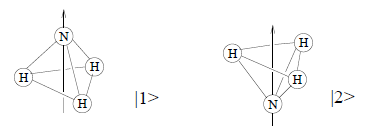
\includegraphics[scale=0.8]{quantica-img/estado.png}
\end{figure}
Suponha que eles estão ortonormalizados, $\langle i | j \rangle = \delta ij $ e que apenas esses dois estados sejam acessíveis ao sistema, de forma que podemos descrevê-lo usando a base formada por $|1\rangle$ e $|2\rangle$. Nessa base, o hamiltoniano $H$ do sistema é dado por

$$
H=\left(\begin{array}{cc}
E_{0} & -E_{1} \\
-E_{1} & E_{0}
\end{array}\right)
$$


a) Se inicialmente o sistema estiver no estado $|1\rangle$, ele permanecerá no estado $|1\rangle$ em um instante posterior? E se estiver no estado $|2\rangle$, ele permanecerá no estado $|2 \rangle$?
b) Ache os autovalores $E_{I}$ e $E_{II}$ e os respectivos autovetores $|I\rangle$ e $|II\rangle$ de $H$, expressando-os em termos de $|1\rangle$ e $|2\rangle$.
c) Baseado no resultado acima, podemos prever pelo menos uma frequência de emissão de radiação eletromagnética possível para uma molécula de amônia. Qual é essa frequência?
d) Ache a probabilidade de medirmos uma energia $E_{I}$ no seguinte estado
$$
|\psi\rangle=\frac{1}{\sqrt{5}}|1\rangle-\frac{2}{\sqrt{5}}|2\rangle
$$



\item Uma partícula quântica de massa $m$ está sujeita a um potencial

$$
V=\frac{1}{2} m \omega^{2}\left(x^{2}+y^{2}+z^{2}\right)
$$


  a) Obtenha os níveis de energia dessa partícula. Isto é, determine os autovalores de
  $$
  -\frac{\hbar^{2}}{2 m} \nabla^{2} \psi+V \psi=E \psi
  $$

  b) Considere o estado fundamental e os dois primeiros níveis excitados. Monte uma tabela mostrando para cada um desses três níveis, o valor da energia, a degenerescência e os respectivos estados em termos dos números quânticos.

  c) Utilizando
  $$
  \nabla^{2} \psi=\left[\frac{1}{r^{2}} \frac{\partial}{\partial r}\left(r^{2} \frac{\partial \psi}{\partial r}\right)-\frac{L^{2}}{\hbar^{2} r^{2}} \psi\right]
  $$
  e lembrado que $L^{2} Y_{\ell m}=\hbar^{2} \ell(\ell+1) Y_{\ell m}$, escreva a equação diferencial do item (a) para a parte radial da função de onda (não é preciso resolvê-la). Identifique nessa equação o potencial efetivo $V_{ef}(r)$.

  d) Resolva a equação diferencial do item anterior para o caso em que $\ell = 0$ e determine o autovalor correspondente. Para isso, admita uma solução do tipo $e^{\alpha r^{2}}$ e determine $\alpha$.




\item Uma partícula de massa $m$ confinada em um poço de potencial unidimensional possui função de onda dada por:

$$
\psi(x) = \left\{\begin{array}{l l l} 0  \  & para \ x < - L/2 \\     A \ cos \frac{3\pi x}{L}  \ & para \ -L/2 < x < L/2  \\ 0 \ & para \ x > L/2 \end{array}\right.
$$


  a) (a) Calcule a constante de normalização $A$.
  b) Calcule a probabilidade de encontrar a partícula no intervalo entre $-L/4 < x < L/4$ .
  c) Através da solução da equação de Schrödinger independente do tempo para esta partícula no referido poço de potencial, ache a energia correspondente à função de onda, em termos de $m$, $L$ e $h$.
  d) Calcule o comprimento de onda do fóton emitido na transição desta partícula para o estado fundamental, em termos de $m$, $L$ e $h$.





\item Considere um oscilador harmônico (em uma dimensão, $x$) de massa $m$ e frequência $\omega$. No instante $t = 0$, o estado do oscilador é $| \psi (0)\rangle = \sum_{n} c_{n} |\phi_{n}\rangle$ onde os $|\phi \rangle$ são os estados estacionários, isto é, $H | \phi \rangle = E_{n}| \phi_{n} \rangle $, sendo $H$ a hamiltoniana e $E_{n} = (n + 1/2)\hbar \omega$ com $n = 0,1,2,...$.


  a) Considerando que os estados $|\phi \rangle$ são normalizados, determine a condição que os coeficientes $c_{n}$ devem satisfazer para que o estado $| \psi (0)\rangle$ seja também normalizado. Calcule, então, a probabilidade $P$ de que uma medida da energia do oscilador, feita num instante $t$ posterior, dê um resultado maior que $2\hbar \omega$.
  b) Se apenas $c_{0}$ e $c_{1}$ são diferentes de zero, dê a expressão para o valor esperado da energia, $\langle H \rangle$, em termos de $c_{0}$ e $c_{1}$. Com a condição $\langle H \rangle = \hbar \omega$, calcule $|c_{0}|^{2}$ e $|c_{1}|^{2}$.
  c) O vetor de estado $|(0)\rangle$ está definido a menos de um fator de fase global, o que nos permite escolher $c_{0}$ real e positivo. Fazendo isso, escrevendo $c_{1} = |c_{1}|e^{i \theta_{1}}$ e mantendo a condição $\langle H \rangle = \hbar \omega$, determine $\theta_{1}$ de modo que $ \langle X \rangle = \frac{1}{2} \sqrt{\frac{\hbar}{m\omega}}$.

      \textbf{Observação}: Lembremos que o efeito do operador posição $X$ sobre os estados estacionários do oscilador harmônico é
        $$
        X\left|\phi_{n}\right\rangle=\sqrt{\frac{\hbar}{2 m \omega}}\left[\sqrt{n+1}\left|\phi_{n+1}\right\rangle+\sqrt{n}\left|\phi_{n-1}\right\rangle\right]
        $$
      entendendo-se que o segundo termo acima é nulo para $n = 0$.
  d) Com $| (0) \rangle$ determinado conforme o item anterior, escreva $|\psi(t) \rangle$ para $t > 0$ e calcule $\langle X \rangle (t)$.




\item Sejam $\vec{L}$, $\vec{R}$ e $\vec{P}$ os operadores do momento angular, da posição e do momento linear, respectivamente.


a) Usando as relações de comutação $\left[L_{i}, L_{j}\right]=i \hbar \sum_{k} \epsilon_{i j k} L_{k}$, mostre que
$$
\vec{L} \times \vec{L}=i \hbar \vec{L}
$$

b) Com a definição $\vec{L} = \vec{R} \times \vec{P}$ e usando $\left[R_{i}, P_{j}\right]=i \hbar \delta_{i j}$, mostre que
$$
\left[L_{i}, R_{j}\right]=i \hbar \sum_{k} \epsilon_{i j k} R_{k}
$$

c) Sabendo que os operadores $\vec{R}$ e $\vec{P}$ são hermitianos, isto é, $R^{\dagger}_{i} = R_{i}$ e $P^{\dagger}_{i} = P_{i}$, mostre que
as componentes do operador do momento angular $\vec{L} = \vec{R} \times \vec{P}$ também são operadores hermitianos.

\textbf{Observação}: Nas expressões acima,$\epsilon_{i j k}$ é o tensor completamente antissimétrico, isto é:

$$
\psi(\epsilon_{ijk}) = \left\{\begin{array}{l l l} 0   &  \mbox{ se houver índices iguais;} \\     +1  \ & \mbox{ se $ijk$ for 123, 231 ou 312;}  \\ -1  & \mbox{ nos demais casos.} \end{array}\right.
$$

Se precisar, use a identidade \[ \sum_{i, j} \epsilon_{i j k} \epsilon_{i j l}=2 \delta_{k l} \]





\item Uma partícula de massa $m$ executa oscilações harmônicas, em uma dimensão, num potencial $U(x) = m \omega^{2}x^{2}/2$. Considere a partícula num estado cuja função de onda é $\psi(x) = Ae^{-bx^{}2}$, onde $A$ e $b$ são constantes.

a) Escreva a equação de Schrödinger independente do tempo para este potencial.
b) Determine o valor de $b$ para que $\psi(x)$ seja solução desta equação de Schrödinger, e o valor da energia associada a esta função de onda.
c) Calcule a constante de normalização $A$.
d) Classicamente, esta partícula oscilaria dentro do intervalo simétrico $[-x_{max},x_{max}]$, onde $x_{max} = [\hbar/m\omega]^{1/2}$. Calcule, usando a Mecânica Quântica, a probabilidade de se encontrar esta partícula no intervalo $[-x_{max},x_{max}]$. Compare este resultado com o esperado pela Mecânica Clássica.





\item Uma partícula de massa $m$ está num potencial tal que a equação de Schrödinger ($com \hbar = 1$) no espaço dos momentos ´
$$
\left(\frac{\vec{p}^{2}}{2 m}-a \nabla_{p}^{2}\right) \bar{\psi}(\vec{p}, t)=i \frac{\partial}{\partial t} \bar{\psi}(\vec{p}, t)
$$
onde
$$
\nabla_{p}^{2}=\frac{\partial^{2}}{\partial p_{x}^{2}}+\frac{\partial^{2}}{\partial p_{y}^{2}}+\frac{\partial^{2}}{\partial p_{z}^{2}}
$$

a) Escreva a equação de Schrödinger no espaço das coordenadas.
b) Qual é o potencial $V (r)$, $r = |\vec{r}|$?
c) Qual é a força, $\vec{F}(\vec{r})$, sobre a partícula?




\item Os operadores de spin de uma partícula de spin$-1$ (um tripleto) podem ser representados no espaço complexo $\mathbb{C}^{3}$ pelas matrizes

$$
\hat{S}_{x}=\frac{\hbar}{\sqrt{2}}\left(\begin{array}{ccc}
0 & 1 & 0 \\
1 & 0 & 1 \\
0 & 1 & 0
\end{array}\right), \hat{S}_{y}=\frac{\hbar}{\sqrt{2}}\left(\begin{array}{ccc}
0 & -i & 0 \\
i & 0 & -i \\
0 & i & 0
\end{array}\right), \hat{S}_{z}=\hbar\left(\begin{array}{ccc}
1 & 0 & 0 \\
0 & 0 & 0 \\
0 & 0 & -1
\end{array}\right)
$$


a) Mostre que as relações de comutação $\left[\hat{S}_{x}, \hat{S}_{y}\right]=i \hbar \hat{S}_{z}$, e permutações cíclicas em $x$, $y$, $z$, são satisfeitas.
b) Se uma medida da componente $z$ do spin é feita, quais são os possíveis resultados? Encontre os respectivos autovetores.
c) Se o estado da partícula é dado pelo vetor
$$
|\phi\rangle=\left(\begin{array}{c}
1 \\
i \\
-2
\end{array}\right),
$$
quais são as probabilidades de se obter cada um dos resultados possíveis das medidas do spin ao longo do eixo$-z$?
d) A partir do resultado do item c), qual é a probabilidade de se encontrar a partícula em qualquer um desses estados?






\item Considere um elétron que se encontra confinado dentro de um poço de potencial unidimensional $V(x)$ dado por
$$
V(x)=\left\{\begin{array}{cc}
+\infty & , x<0 \\
0 & , 0<x<d \\
+\infty & , x>d
\end{array}\right.
$$

a) Escreva a equação de Schrödinger para este elétron e as condições de contorno que devem ser satisfeitas pelas funções de onda.
b) Obtenha as funções de onda normalizadas e determine os valores das energias permitidas para este elétron.

Admita agora que este elétron se encontre no estado quântico cuja função de onda dentro do poço é dada por
$$
\psi(x)=\sqrt{\frac{2}{d}} \operatorname{sen}\left(\frac{3 \pi x}{d}\right).
$$

c) Determine o número quântico n do estado ocupado por este elétron e seu comprimento de onda nesse estado.
d) Determine a probabilidade de encontrar este elétron entre $x = 0$ e $x = d/6$.



\item A equação de Schrödinger independente do tempo para o problema unidimensional de uma partícula de massa m sujeita a um potencial de oscilador harmônico é

$$
\left(-\frac{\hbar^{2}}{2 m} \frac{d^{2}}{d x^{2}}+\frac{1}{2} m \omega^{2} x^{2}\right) \psi_{n}(x)=E_{n} \psi_{n}(x), \quad n=0,1,2, \ldots
$$

onde $\omega$ é a frequência angular do oscilador. Um método para se resolver essa equação consiste em expressá-la em termos do operador

$$
a=\frac{1}{\sqrt{2}}\left(\sqrt{\frac{m \omega}{\hbar}} x+\sqrt{\frac{\hbar}{m \omega}} \frac{d}{d x}\right)
$$
e de seu conjugado hermitiano.

a) A função de onda do estado fundamental do oscilador satisfaz a equação diferencial a $\psi_{0}(x ) = 0$. Resolva esta última equação e determine $\psi_{0}(x)$ a menos de uma
constante multiplicativa.
b) Calcule essa constante normalizando $\psi_{0}(x)$.
c) Obtenha o valor da energia do estado fundamental desse oscilador.
d) Suponha, agora, que o oscilador seja perturbado pelo potencial
$$
V(x)=V_{0} \exp \left(-x^{2} / b^{2}\right)
$$
onde $V_{0}$ e $b$ são constantes reais. Usando teoria de perturbações de primeira ordem, calcule o deslocamento de energia do estado fundamental.



\item Uma partícula de spin $\frac{1}{2}$ tem momento de dipolo magnético $\vec{\mu} = \gamma \vec{S}$, onde $\gamma$ é uma constante real e $\vec{S} = \frac{\hbar}{2} \vec{\sigma}$ é o operador de spin, sendo
$$
\sigma_{x}=\left(\begin{array}{ll}
0 & 1 \\
1 & 0
\end{array}\right), \quad \sigma_{y}=\left(\begin{array}{cc}
0 & -i \\
i & 0
\end{array}\right), \quad \sigma_{z}=\left(\begin{array}{cc}
1 & 0 \\
0 & -1
\end{array}\right)
$$
as matrizes de Pauli. Se essa partícula está imersa num campo magnético uniforme $\vec{B}$, o hamiltoniano que governa a dinâmica do spin é $H = - \vec{\mu} \cdot \vec{B}$. No que segue, suponha que o campo magnético esteja na direção do eixo $Oz$.

a) Dê a forma explícita do operador hamiltoniano como uma matriz $2 \times 2$, em termos de $\gamma$, $\hbar$ e $B$.
b) Escreva as expressões para os estados estacionários como vetores-coluna normalizados e indique suas respectivas energias.
$$
\chi(0)=\frac{1}{\sqrt{2}}\left(\begin{array}{l}
1 \\
e^{i \alpha}
\end{array}\right) \quad \mbox{com $\alpha$ real}
$$
Qual será o estado de spin, $\chi (t)$, num instante $t$ posterior?
c) No instante inicial, $t = 0$, a partícula é preparada no estado de spin
d) Nesse instante posterior é feita uma medida de $Sx$, a componente do spin segundo o eixo $Ox$. Qual a probabilidade $P_{+}(t) $ de se obter o valor $+ \hbar / 2$?




\item Considere o problema unidimensional quântico de uma partícula de massa m sujeita ao
potencial
$$
V(x)=\left\{\begin{array}{cc}
+\infty & , x<0 \\
0 & , 0<x<a \\
+\infty & , x>a
\end{array}\right.
$$

a) Escreva a equação de Schrödinger independente do tempo para este problema.
b) Resolva a equação, achando todas as soluções aceitáveis independentes. Isto é: determine todos os valores possíveis para a energia, $E_{n}$, e as funções de onda normalizadas correspondentes, $\psi_{n}(x)$.

Suponha agora que, na verdade, o potencial total tenha a forma $V_{total}(x) =V(x) +W(x)$, sendo $W(x)$ uma pequena correção dada por
$$
W(x)=\left\{\begin{array}{cc}
0 & , x<0 \\
W_{0} sen (\pi x /a) & , 0<x<a \\
+\infty & , x>a
\end{array}\right.
$$
c) Usando teoria de perturbações de primeira ordem, calcule a correção para a energia do estado fundamental obtida no item anterior.




\item Para uma partícula de spin $\frac{1}{2}$ o operador de spin é dado por $\vec{S} = \frac{\hbar}{2} \vec{\sigma} $, onde
$$
\sigma_{x}=\left(\begin{array}{ll}
0 & 1 \\
1 & 0
\end{array}\right), \quad \sigma_{y}=\left(\begin{array}{cc}
0 & -i \\
i & 0
\end{array}\right), \quad \sigma_{z}=\left(\begin{array}{cc}
1 & 0 \\
0 & -1
\end{array}\right)
$$
são as matrizes de Pauli. Seja $\hat{n}$ o vetor unitário na direção de ângulos ($\theta$, $\phi$), conforme ilustra a figura abaixo.
\begin{figure}
  \centering
  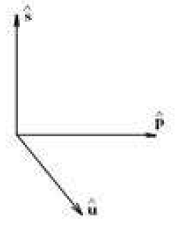
\includegraphics[scale=0.8]{quantica-img/vetor.png}
\end{figure}



a) Calculando o produto escalar, mostre explicitamente que o operador que representa a componente do spin nessa direção, $ \vec{S} = \frac{\hbar}{2} \vec{\sigma} $, é dado por
$$
S_{n}=\frac{\hbar}{2}\left(\begin{array}{cc}
\cos \theta & e^{-i \phi} \operatorname{sen} \theta \\
e^{i \phi} \operatorname{sen} \theta & -\cos \theta
\end{array}\right)
$$
b) Mostre que os únicos valores que podem ser obtidos numa medida de $S_{n}$ são $+\hbar / 2$ e $- \hbar/2$, qualquer que seja a direção $\hat{n}$.
c) Obtenha o vetor coluna normalizado que representa o estado no qual uma medida de $S_{n}$ produz necessariamente o valor $+\hbar/2$. Simplifique a resposta final expressando a dependência em $\theta$ em termos de $sen(\theta/2)$ e $cos(\theta/2)$.
d) Suponha, agora, que $\theta = 60º$ e $\phi = 45º$. Se a partícula for preparada de tal forma que a componente $z$ do spin, $S_{z}$, tenha o valor bem definido $+\hbar/2$, qual é a probabilidade de obter-se esse mesmo valor numa medida de $S_{n}$? \textit{Dê a resposta numérica}.






\item Considere uma partícula de massa $m$ na presença de um potencial harmônico $V(x) = \frac{1}{2} m \omega^{2}x^{2}$, onde $\omega$ é a frequência angular do oscilador e $x$ é a coordenada da partícula (1-dim).

a) São dadas as funções de onda estacionárias correspondentes ao estado fundamental $\psi_{0}$ e ao primeiro estado excitado $\psi_{1}$:
$$
\psi_{0}(x) = A \ exp \left(- \frac{m \omega}{2 \hbar} x^{2}  \right) \ , \  \  \psi_{1}(x) = B \ x \ exp \left(- \frac{m \omega}{2 \hbar} x^{2}  \right) \ ,
$$
onde $A$ e $B$ são constantes de normalização. Calcule $A$ e $B$ supondo que as funções de onda sejam reais.
b) Seja $E_{0}$ a energia do estado fundamental. Sabemos que $E_{1} = E_{0} + \hbar \omega$ para o primeiro estado excitado, já que o quantum de energia do oscilador é $\hbar \omega$. Usando a equação de Schrödinger, encontre a energia $E_{0}$.
c) Para os estados estacionários, o valor médio da posição $\langle x \rangle$ é sempre nulo. Construa uma função de onda não estacionária como combinação linear de $\psi_{0}$ e $\psi_{1}$ com coeficientes reais, tal que o valor médio $\langle x \rangle$ seja o maior possível. Em outras palavras, considere o estado normalizado
$$
\psi(x) = \sqrt{1 - \beta^{2}} \psi_{0} (x) + \beta \psi_{1} (x),
$$
com $0 \leq \beta^{2} \leq 1$ e determine o coeficiente $\beta$ que maximiza o valor de $\langle x \rangle$.
d) Suponha que a função de onda construída no item anterior descreva o estado do oscilador harmônico no tempo $t = 0$. Escreva a função de onda do estado para um tempo $t > 0$ arbitrário, supondo que nenhuma medição foi feita sobre o sistema. Para esse estado, avalie o valor médio da posição $\langle x \rangle (t)$ em função do tempo.




\item Seja uma partícula com momento angular $\ell = 1$.

a) Na representação onde as matrizes de $\mathbf{L}^{2}$ e $\mathbf{L}_{z}$ são diagonais, obtenha a matriz da componente $\mathbf{L}_{x}$. Lembre que a matriz de $\mathbf{L}_{x}$ deve representar um operador hermitiano. Sugerimos usar os operadores escada $\mathbf{L}_{\pm}$.
b) Calcule os autovalores de $\mathbf{L}_{x}$.
c) Encontre o autovetor de $\mathbf{L}_{x}$ com o maior autovalor.
d) Suponha agora que você encontrou o maior autovalor numa medição de $\mathbf{L}_{x}$. Calcule as probabilidades de medir respectivamente $+\hbar$, 0 e $-\hbar$  numa medição posterior de $\mathbf{L}_{z}$.



\item Seja a função de onda de uma partícula em uma dimensão, dada por $\psi(x,t)$. A densidade de probabilidade $\rho(x,t)$ é definida como $\rho(x,t) = \psi^{*}(x,t) \psi(x,t)$. O valor de $\rho(x,t)$ pode mudar no tempo devido ao fluxo de probabilidade saindo ou entrando na região, que se pode expressar como uma equação de continuidade,
$$
\frac{\partial \rho}{\partial t} = - \frac{\partial j}{\partial x},
$$
onde $j(x,t)$ é a densidade de corrente de probabilidade.


  a) Dada a equação de Schrodinger,
  $$
  i \hbar \frac{\partial \psi}{\partial t} = \left[ \frac{- \hbar^{2}}{2m} \frac{\partial^{2}}{\partial x^{2}} + V(x) \right] \psi ,
  $$
  escreva a derivada temporal de $\rho(x,t)$ em termos de $\psi$, $\psi^{*}$ e suas derivadas espaciais.
  b) Obtenha a forma explícita de $j(x,t)$.
  c) Ache a equação relacionando a derivada do valor esperado da posição, $\frac{d \langle x \rangle}{d t}$, com o valor esperado do momento, $\langle p \rangle$. \textit{Dica:} use integração por partes e assuma que as funções $\psi$  e sua derivada, $\frac{\partial \psi}{\partial x}$, vão ao infinito mais rápido do que $\frac{1}{x}$.



\item Seja o seguinte hamiltoniano representativo de um sistema físico:
$$
\hat{H} = \hbar \omega_{0} \left( \hat{a}^{\dagger} \hat{a} + \frac{1}{2} \right).
$$
Os autoestados deste hamiltoniano são denominados $| n \rangle$, são não-degenerados e satisfazem $\hat{N}|n\rangle = n|n\rangle$, onde $n$ é um número inteiro e $\hat{N} \equiv \hat{a}^{\dagger} \hat{a}$.


  a) Assuma que os operadores $\hat{a}$ e $\hat{a}^{\dagger}$ obedecem à relação de comutação $[\hat{a}, \hat{a}^{\dagger}] = 1$. Mostre que os estado $\hat{a}|n\rangle$ e $\hat{a}^{\dagger} |n\rangle$ são autoestados de $\hat{N}$, usando as relações de comutação. Determine os autovalores correspondentes a estes estado, $n'$ e $n"$, respectivamente.
  b) Dado que todos os estado $|n\rangle$ são não degenerados, determine a constante de proporcionalidade entre os estados $\hat{a}|n\rangle$ e os estados $|n'\rangle$ encontrado no item (a). \textit{Dica:} lembre que todos os estados são normalizados. Assuma que o valor esperado do hamiltoniano em qualquer de seus autoestados seja positivo, $\langle H \rangle \geq 0$, e que $\hat{a}|0\rangle = 0$. O que se pode concluir sobre o número de estados $|n\rangle$; ele é finito ou infinito?
  c) Assuma agora que os operadores $\hat{a}$ e $\hat{a}^{\dagger}$ obedecem à relação de anticomutação $\{ \hat{a}, \hat{a}^{\dagger} \} = \hat{a}\hat{a}^{\dagger} + \hat{a}^{\dagger} \hat{a} = 1$. Mostre que os estados $\hat{a}|n\rangle$ e $\hat{a}^{\dagger}|n\rangle$ são autoestados de $\hat{N}$, usando as relações de anticomutação, e determine os autovalores $n'$ e $n"$ correspondentes a estes estados. Dado que todos os estados $|n\rangle$ são não degenerados, determine a constante de proporcionalidade entre os estados $\hat{a}|n\rangle$ e esses estados $|n'\rangle$. \text{Dica}: lembre que todos os estados são normalizados.
  d) Assumindo, como no item (c), que os operadores $\hat{a}$ e $\hat{a}^{\dagger}$ obedecem à relação de anticomutação, que o valor esperado do hamiltoniano em que qualquer de seus autoestados seja positivo, $\langle H \rangle \geq 0$, e que $\hat{a}|0\rangle = 0$, isto implica que o número de estados $|n\rangle$ é finito. Quais são estes únicos estados $|n\rangle$ não nulos neste caso?



\item Um elétron de massa $m$ está confinado numa esfera de raio $a$, isto é, submetido ao potencial $V(r) = 0$ para $r < a$ e $V (r) = \infty$ para $r > a$.

a) Escreva a equação de Schrödinger independente do tempo para a função $u(r) = rR(r)$, sendo $\psi(r,\theta,\phi) = R(r) Y_{l,m}(\theta,\phi)$ a função de onda completa desse elétron.
b) Imponha a devida condição de contorno e encontre, para o estado fundamental, $\psi(r,\theta,\phi)$ e a respectiva energia.
c) Escreva a energia do estado fundamental em termos do volume da esfera, massa do elétron e constantes fundamentais.
d) Encontre a pressão exercida por esse elétron na superfície da esfera. Expresse em termos da massa $m$, raio $a$ e constantes universais.



\item Duas partículas com spin $1/2$ se aproximam e interagem segundo o hamiltoniano
$$
H = \frac{4a(t)}{\hbar} \vec{S}_{1} \cdot \vec{S}_{2},
$$
sendo $a(t) = a_{0}$, constante, para $0 < t < \tau$ e $a(t) = 0$ para $t < 0$ e $t > \tau$. Em $t = - \infty$ o estado do sistema é $|+, - \rangle$, sendo $|\pm \rangle$ autovetores do operador $S_{i,z}$ com autovalores $\pm \hbar / 2$.

a) Escreva a matriz $H$ na base dos autovetores de $S_{1,z}$ e $S_{2,z}$.
b) Determine os autovalores e autovetores de $H$.
c) Qual é o estado $|\psi \rangle$ do sistema para $0 < t < \tau$?
d) Qual é o estado $|\psi \rangle$ do sistema para $t > \tau$ qualquer?
e) Qual a probabilidade de uma medida de $S_{1,z}$ fornecer o valor $\hbar/2$ para $t > \tau$?
f) Após $\Delta t$ segundos dessa medida, qual a probabilidade de uma medida de $S_{2,z}$ dar o valor $-\hbar/2$?



\item Uma partícula de massa $m$ encontra-se inicialmente em um poço de potencial unidimensional dado por
$$
V(x)=\left\{\begin{array}{cc}
+\infty, &  x \leq \frac{L}{2}, \\
0, &  -\frac{L}{2} <x<  \frac{L}{2},\\
+\infty, &  x \geq \frac{L}{2}.
\end{array}\right.
$$

a) Calcule as autofunções e as autoenergias do estado fundamental e do primeiro estado excitado.
b) Considere agora que o potencial expande-se instantaneamente para
$$
V(x)=\left\{\begin{array}{cc}
+\infty, &  x \leq L, \\
0, &  -L <x<  L,\\
+\infty, &  x \geq L.
\end{array}\right.
$$
Calcule a probabilidade da partícula realizar uma transição do estado fundamental do potencial (1) para o primeiro estado excitado do potencial (2).
c) Calcule a probabilidade da partícula continuar no estado fundamental após a expansão.
d) Considere que a partícula se encontre no estado fundamental após a expansão. Calcule a probabilidade da partícula ser encontrada fora da região $-L/2 < x < L/2$.




\item As matrizes de Pauli, $\sigma_{x}$, $\sigma_{y}$ e $\sigma_{z}$, são extremamente importantes quando se considera uma partícula de spin 1/2.

a) Utilize explicitamente a representação matricial dos operadores de Pauli e encontre seus autovalores e autovetores, bem como o comutador [$\sigma_{y}, \sigma_{x}$].
b) Considere um estado arbitrário para uma partícula de spin 1/2 dado por $|\psi \rangle = a|-\rangle + b|+\rangle$, com $|a|^{2} + |b|^{2} = 1$, sendo $\{|-\rangle,|+\rangle \}$ autovetores de $\sigma_{z}$. Mostre como este estado é transformado sob a ação de cada um dos operadores  $\sigma_{x}$, $\sigma_{y}$ e $\sigma_{z}$, independentemente.
c) Mostre como o operador $exp(i \alpha \sigma_{x})$ atua sobre o estado $|\psi \rangle$.
d) Quais imposições devem ser consideradas sobre $\alpha$ para que o operador do item (c) seja hermitiano? e para que seja unitário?



\item O hamiltoniano de um sistema quântico de dois níveis é representado por:
$$
\hat{H} = \left(
  \begin{array}{cc}
    \varepsilon & \lambda \\
    \lambda & \varepsilon \\
  \end{array}
\right)
$$
No instante $t = 0$, o sistema se encontra no estado representado por $\left( \begin{array}{c} 1 \\ 0 \\ \end{array} \right)$.

  a) obtenha os autoestados e respectivos autovalores do hamiltoniano.
  b) Mostre que a probabilidade de encontrar o sistema no mesmo estado inicial, para $t > 0$, varia harmonicamente com $t$, com frequência que tende a zero quando $\lambda \rightarrow 0$.



\item Considere uma partícula de massa $m$ movendo-se em uma dimensão, propagando-se ao longo do eixo $x$, no seu sentido positivo, em um potencial do tipo delta de Dirac
$$
V(x) = -q \delta(x), \quad \quad (q>0)
$$

  a) Quais as condições de continuidade que a função de onda deve satisfazer em $x=0$?
  b) Encontre as funções de onda.
  c) Encontre os coeficientes de transmissão e reflexão.



\item Um elétron no campo coulombiano de um próton encontra-se em um estado descrito pela função de onda
$$
\psi(\vec{r}) = \frac{1}{\sqrt{11}} \left[ \frac{1+i}{\sqrt{2}} \psi_{311}(\vec{r}) + \psi_{21-1}(\vec{r}) + 3\psi_{210}(\vec{r})   \right]
$$
onde $\psi_{nlm}(\vec{r}) = R_{nl}(r) Y_{lm}(\theta, \phi)$ são as autofunções do hamiltoniano $H$ do sistema, cujos autovalores são dados por
$$
E_{n} = \frac{-e^{}2}{2a_{0}} \frac{1}{n^{2}},
$$
onde $e$ e $a_{0}$ são, respectivamente, a carga do elétron e o raio de Bohr. Além disso, $Y_{lm}(\theta, \phi)$ são autofunções do quadrado do momento angular, $L^{2}$, e da sua componente $L_{z}$, com autovalores $\ell(\ell + 1) \hbar^{2}$ e $m\hbar$, respectivamente.

  a) $\psi(\vec{r})$ é uma autofunção de H? Se é, qual é o autovalor correspondente de H? Se não, qual é o valor esperado de H?
  b) $\psi(\vec{r})$ é uma autofunção de $L^{2}$? Se é, qual é o autovalor correspondente? Se não, qual é o valor esperado de $L^{2}$?
  c) $\psi(\vec{r})$ é uma autofunção de $L_{z}$? Se é, qual é o autovalor correspondente? Se não, qual é o valor esperado de $L_{z}$?
  d) Calcule as probabilidades do elétron se encontrar em um estado com $\ell = 1$ e projeções $m = 1, 0,-1$, respectivamente.
  e) Adotando a função de onda dada como estado inicial para $t=0$, obtenha $\Psi(\vec{r},t)$.




\item Um rotor quântico, cuja orientação está especificada somente pela coordenada $\phi$, é descrito pelo hamiltoniano
$$
H = CH^{(0)} + BV(\phi)
$$
onde $H^{(0)} = -\hbar^{2} \frac{d^{2}}{d \phi^{2}}$, $V(\phi) = \hbar^{2} \operatorname{sen} 2\phi$ e $C>>B$. Sabendo que os autovalores e os autoestados de $H^{(0)}$ sao, respectivamente, $\phi_{m}(\phi) = \frac{e^{i m \phi}}{\sqrt{2\pi}}$ e $E_{m} = C \hbar^{2} m^{2}$ com $m = 0, \pm 1, \pm 2, \dots$, pede-se:

  a) A correção não nula de mais baixa ordem para a energia do estado fundamental.
  b) A correção não nula de mais baixa ordem para a função de onda do estado fundamental.





\item Um átomo de gás nobre exerce um potencial atrativo sobre um elétron, de massa $m$, não ligado. Este potencial pode ser aproximado pelo seguinte poço de potencial unidimensional:
$$
V(x)=\left\{\begin{array}{cccc}
0 & \mbox{para} & x < L & \mbox{região 1} \\
-V_{0} & \mbox{para} &  0 \leq x \leq  L & \mbox{região 2} \\
0 & \mbox{para} & x > L &  \mbox{região 3}.
\end{array}\right.
$$

  a) Esboce o poço de potencial e mostre a energia do elétron no seu diagrama.
  b) Encontre a energia cinética e o comprimento de onda de De Broglie do elétron nas três regiões.
  c) Dado que a função de onda do elétron é da forma
  $$
    \phi(x)=\left\{\begin{array}{cccc}
    A e^{ik_{1}x} + B e^{-ik_{1} x } & \mbox{para} & x < L \\
    F e^{ik_{2}x} + G e^{-ik_{2} x } & \mbox{para} & 0 \leq x \leq  L \\
    C e^{ik_{3}x} + D e^{-ik_{3} x } & \mbox{para} & x > L ,
    \end{array}\right.
  $$
  utilize as condições que devem ser satisfeitas pela função de onda, nos contornos do potencial ($x=0$ e $x=L$), e obtenha o conjunto de equações que definem as relações entre as constantes $A$, $B$, $C$, $D$, $F$ e $G$. \textbf{Não é necessário encontrar os valores de cada um desses coeficientes, exceto para aqueles que devem ser nulos por considerações físicas}.
  d) Sabendo que
  $$
  \frac{A}{C} = e^{ik_{1}L} \left[ \operatorname{cos}k_{2}L - \frac{i}{2} \left( \frac{k_{1}}{k_{2}} + \frac{k_{1}}{k_{2}} \right) \operatorname{sen} k_{2} L   \right],
  $$
  obtenha a expressão para o coeficiente de reflexão na região 1.
  e) É possível para o elétron se movimentar, na região do potencial atômica, sem sofrer reflexão? Se sim, sob que condições isso ocorre? Se não, porque não?


\item Se escolhermos um sistema onde $\hbar = m = \omega = 1$, com $m$ e $\omega$ sendo a massa e a frequência angular de uma partícula sob ação de um potencial do tipo oscilador harmônico simples, as autofunções do hamiltoniano e seus respectivos autovalores são:
$$
\psi_{n} (x) = \frac{(2)^{- \frac{n}{2}}}{\pi^{\frac{1}{4}}} (n!)^{\frac{1}{2}} H_{n} (x) e^{- \frac{x^{2}}{2}}
$$
$$
E_{n} = n + \frac{1}{2},
$$
onde $H_{n}(x)$ são os \textit{polinômios de Hermite} de ordem $n (n=1,2,3, ...)$.

No instante $t=0$ o oscilador harmônico está em um estado descrito pela seguinte função não normalizada:
$$
\phi(x,0) = (1+x)e^{\frac{-x^{2}}{2}}
$$

  a) Escreva o estado $\phi(x,0)$ em termos dos polinômios de Hermite.
  b) Escreva o estado $\phi(x,0)$ em termos das autofunções normalizadas do oscilador harmônico simples.
  c) Escreva a equação de Schrödinger dependente do tempo e encontre a função de onda normalizada $\phi(x,t)$ para um instante $t$ genérico e mostre que ela é dada por
  $$
  \phi(x,t) = \sqrt{\frac{2}{3 \pi^{1/2}}} e^{-x^{2}/2} \left\{  e^{-it/2} + x e^{-3it/2}   \right\}
  $$
  d) Determine o valor esperado da coordenada $x$ como função do tempo.
  e) Considere que o oscilador harmônico seja perturbado pelo potencial
  $$
  \hat{W} = \lambda \hat{x},
  $$
  obtenha a primeira correção não nula de $E_{n}$, para qualquer $n$.




\item Prove que se $\hat{A}$ e $\hat{B}$ são dois operadores que comutam entre si, com autovalores não degenerados, então eles possuem um conjunto de autofunções simultâneas.




\item a) Dê a definição de um operador hermitiano.

  b) Sejam dois operadores hermitianos $\hat{C}$ e $\hat{D}$ que satisfazem a relação de comutação $ \left[ \hat{C}, \hat{D} \right] = i \hat{F}$, onde $\hat{F}$ é também um operador hermitiano. Se $\Delta \hat{A} = \hat{A} - \langle \hat{A} \rangle$, onde $\langle \hat{A} \rangle$ é o valor médio do operador $\hat{A}$ em um estado $\psi$. Dê a definição de valor médio de um operador e mostre que $\left[ \Delta \hat{C}, \Delta \hat{D} \right] = i \hat{F}$.
  c) Mostre que $\hat{C}$ e $\hat{D}$ satisfazem a relação de incerteza
  $$  \left\langle \left( \hat{C} - \langle \hat{C} \rangle \right)^{2} \right\rangle   \left\langle \left( \hat{D} - \langle \hat{D} \rangle \right)^{2} \right\rangle    \geq    \frac{1}{4} \langle \hat{F} \rangle^{2}. $$
  Para simplificar, assuma que a função correlação entre $\hat{C}$ e $\hat{D}$ é nula, ou seja, que
  $$
  \left\langle \left[ \Delta \hat{C}, \Delta \hat{D} \right]_{+}  \right\rangle = \left\langle   \Delta \hat{C} \Delta \hat{D} + \Delta \hat{D} \Delta \hat{C} \right\rangle = 0.
  $$
  d) Se $\hat{C} = \hat{x}^{2}$ e $\hat{D} = \hat{p}^{2}_{x}/(2m)$, onde $\hat{x}$ é o operador posição, $\hat{p}$ o operador momento e $m$ a massa da partícula, obtenha a relação de incerteza satisfeita por $\hat{C}$ e $\hat{D}$, sabendo que $\left[\hat{x}, \hat{p}_{x} \right] = i\hbar \hat{I}$.



\item Considere uma partícula em uma dimensão, suficientemente localizada em um intervalo finito de $x$, possuindo função de onda $\psi(x,t)$ e sujeita a um potencial \textit{real} qualquer.

  a) Usando a equação de Schrödinger, mostre que a probabilidade
  $$ P = \int_{-\infty}^{\infty} | \psi (x,t) |^{2} dx $$
  é conservada (sugestão: use integração por partes)
  b) Supondo agora que o potencial possui uma parte imaginária, ou seja
  $$ V(x) = V_{0} + i \Lambda,$$
  onde $V_{0}$ e $\Lambda$ são reais e $\Lambda$ é constante, mostre que
  $$
  \frac{dP}{dt} = -\frac{2 \Lambda}{\hbar} P.
  $$
  c) Resolvendo a equação do item 9b, mostre que a vida média da partícula é $\tau = \hbar/(2 \Lambda)$.



\item Um oscilador harmônico unidimensional, de massa $m$ e frequência $\omega$, está em um estado tal que medidas de energia resultam somente em $\hbar \omega / 2$ e $3 \hbar \omega / 2$, com probabilidades iguais. Estas informações determinam completamente o estado da partícula, a menos de uma fase. Sabendo que no instante $t=0 \ s$ o valor médio do operador momento, $\langle p \rangle$, é $\left[ \frac{m\hbar \omega}{2} \right]^{1/2}$, determine:

  a) a fase e, consequentemente, este estado no instante $t = 0 \ s$;
  b) o valor médio do operador momento $\langle p(t) \rangle$ em um instante $t$ qualquer.




\item Um rotor plano está em um estado descrito pela função de onda normalizada:
$$
\psi (\phi) = \frac{2}{(3\pi)^{1/2}} \operatorname{sen}^{2} \phi.
$$
Determine a probabilidade de encontrar cada um dos autovalores possíveis de $L_{z}$. Ache os valores esperados $\langle L_{z} \rangle$ e $\langle L_{z}^{2} \rangle$. (Sugestão: expresse a função dada em termos das autofunções normalizadas $\phi_{m}$ do operador $L_{z}: L_{z}\phi_{m} = m\hbar \phi_{m}$)



\item Uma partícula em um poço infinito unidimensional, situado no intervalo $0 < x < a$, encontra-se no estado
$$
\phi(x) = Ax(a-x).
$$

  a) Determine a constante de normalização $A$.
  b) Qual é o estado estacionário que mais se aproxima da função $\phi(x)$?
  c) Encontre os valores médios da posição $\langle x \rangle$ e do momento $\langle p \rangle$ em $t=0 \ s$.




\item A hamiltoniana de um oscilador harmônico unidimensional, com massa $m$ e frequência $\omega$, é dada por
$$
H = \frac{p^{2}}{2m} + \frac{1}{2} m \omega^{2} x^{2}.
$$
Classicamente, a energia do estado fundamental de um oscilador harmônico é nula. Quanticamente, ela não é nula. Porque? \\
Estime a energia mínima (estado fundamental) de um oscilador harmônico quântico utilizando a relação de incerteza mínima $\Delta x \Delta p = \frac{\hbar}{2}$.





\item Considere, para um partícula de massa $m$ em uma dimensão, a função de onda
$$
\psi(x) = A \left( \frac{x}{x_{0}} \right)^{n} e^{-x/x_{0}},
$$
onde $A$, $n$ e $x_{0}$ são constantes. Encontre o potencial $V(x)$ e a energia $E$ tais que essa função seja uma auto-função da equação de Schrödinger. Considere que $V(x) \rightarrow 0$ para $x \rightarrow 0$.


\item O primeiro estado excitado de um oscilador harmônico isotrópico de frequência natural $\omega_{0}$, massa $m$ e Hamiltoniano $H_{0}$, em $3-D$, é triplamente degenerado.

  a) Calcule o desdobramento desses níveis devido à pertubação $H' = b(xy + yz)$, sendo $b$ uma constante, em primeira ordem de pertubação.
  b) Determine, em função dos autoestados do oscilador harmônico $3-D$ não perturbado, os autoestados associados aos níveis perturbados.
  \item[] Sugestão: Utilize a representação de números de ocupação $|n_{x}, n_{y}, n_{z} \rangle$, tal que
      $$
      H_{0} | n_{x}, n_{y}, n_{z} \rangle = \left( n_{x} + n_{y} + n_{z} + \frac{3}{2} \right) \hbar \omega_{0} | n_{x}, n_{y}, n_{z} \rangle.
      $$
  \item[] Dado: para estados de um oscilador harmônico em $1-D$, temos a seguinte relação:
  $$
  \langle n | x_{i} | n + 1 \rangle = \sqrt{ \frac{(n+1)\hbar}{2m\omega_{0}} }, \quad \quad x_{i} = x,y,z.
  $$





\item Considere o átomo de hélio ($He$).

a) Escreva o seu hamiltoniano $\hat{H}_{He}$, tratando o núcleo como uma carga pontual de massa infinita.
b) Considere o hamiltoniano do $He$ sem o termo repulsivo intereletrônico como um hamiltoniano de ordem zero $\hat{H}_{0}$. Utilizando resultados para o estado fundamental de um átomo hidrogenóide,
$$
\psi_{1s} = \left(  \frac{z^{3}}{\pi a_{0}^{3}}  \right)^{1/2} \operatorname{exp} (- Zr/a_{0}), \quad E_{1s} = - \frac{Z^{2} e^{2}}{2a_{0}}
$$
determine a autofunção  $\psi(\mathbf{r}_{1},\mathbf{r}_{2})$ e a autoenergia $E_{0}$ correspondentes ao estado fundamental de $\hat{H}_{0}$. Compare a autoenergia com o resultado experimental para o átomo de $He$, $E_{exp} = -78,8 \ eV$.
c) Escreva uma função de estado aproximada para o átomo de $He$,  $\phi_{He}(\mathbf{r}_{1}m_{s1},\mathbf{r}_{2}m_{s2})$, a partir da autofunção do ítem anterior e das funções de spin $\chi_{+}$ e $\chi_{-}$ correspondendo às componentes $m_{s} = +\frac{1}{2}$ e $m_{s} = -\frac{1}{2}$, respectivamente.
d) Obtenha uma melhor aproximação para a energia do estado fundamental do $He$ considerando o termo repulsivo descartado acima como uma perturbação e utilizando teoria de perturbação de primeira ordem.
\item[] Dados:

$$
\left(\frac{z^{3}}{\pi a_{0}^{3}} \right)^{2} \int \int e^{-2z(r_{1}+r_{2})/a_{0}} \frac{e^{2}}{r_{12}} d^{3} r_{1} d^{3} r_{2} = \frac{5Ze^{2}}{8a_{0}}; \quad \quad r_{12} \equiv | \mathbf{r}_{1} - \mathbf{r}_{2}|
$$

$$
\mbox{ Raio de Bohr: } a_{0} = \frac{\hbar^{2}}{m_{e}e^{2}};  \quad \quad \frac{e^{2}}{2a_{0}} = 13,6 eV
$$


\item Considere um sistema quântico descrito por um espaço vetorial de duas dimensões gerado por dois vetores de base ortonormais $|1\rangle$ e $|2\rangle$. Seja $\hat{H}$ o hamiltoniano do sistema, cujos elementos de matriz são
\begin{eqnarray*}
% \nonumber % Remove numbering (before each equation)
\langle 1 | \hat{H} | 1 \rangle & = & \langle 2 | \hat{H} | 2 \rangle  = a \\
\langle 1 | \hat{H} | 2 \rangle  & = & \langle 2 | \hat{H} | 1 \rangle  = b.
\end{eqnarray*}
Considere agora um outro observável $\hat{S}$ cujos elementos de matriz são
\begin{eqnarray*}
% \nonumber % Remove numbering (before each equation)
\langle 1 | \hat{H} | 1 \rangle & = & 1 \\
\langle 2 | \hat{H} | 2 \rangle  & = & -1 \\
\langle 1 | \hat{H} | 2 \rangle  & = & \langle 2 | \hat{S} | 1 \rangle = 0.
\end{eqnarray*}

a) Quais são os autovalores e autovetores de $\hat{H}$?
b) Suponha que o estado do sistema seja $| \psi \rangle = \frac{1}{\sqrt{2}}  \left( |1\rangle + |2\rangle \right)$. Quais os possíveis resultados, com suas respectivas probabilidades, das medidas de $\hat{H}$ e $\hat{S}$?
c) Suponha que em $t = 0$ o sistema esteja no estado $|\psi(0) \rangle = |1\rangle$. Qual o estado para um tempo $t$, $|\psi(t)\rangle$? Para quais instantes de tempo uma medida de $\hat{S}$ fornece o valor $-1$ com $100\%$ de probabilidade?
d) Os operadores $\hat{S}$ e $\hat{H}$ podem ser diagonalizados simultaneamente? Justifique.




\item Um feixe de partículas com spin $1/2$ incide a partir da esquerda no sistema exibido na figura abaixo. Após passar por A, as partículas encontram-se no estado de spin associado ao autovalor $+ \hbar/2$ de $S_{z}$.
\begin{figure}
  \centering
  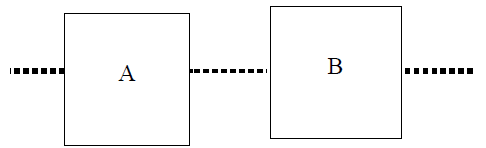
\includegraphics[scale=0.7]{quantica-img/aparato.png}
  %\caption{}\label{}
\end{figure}
Responda justificando:

a) Se o aparato B mede a componente $y$ do spin, quais são os resultados possíveis que B pode fornecer?
b) Qual a probabilidade de B fornecer como resultado $\hbar/2$?





\item Considere os operadores associados ao momento angular orbital $L_{x}$, $L_{y}$ e $L_{z}$. Suponha que o estado do sistema é dado por
$$
\psi = N \left[ (1-i)Y_{3,1} + iY_{2,1} + 2Y_{1,1}  \right].
$$
onde N é uma constante e $Y_{lm}$ são os harmônicos esféricos propriamente normalizados.

a) Encontre $N$ para que $\psi$ esteja normalizada.
b) Este estado é autovetor de $\mathbf{L}^{2}$? Se é, qual é o autovalor correspondente? Se não, qual é o valor esperado (médio) de $\mathbf{L}^{2}$?
c) Qual a incerteza de $L_{z}$ neste estado?
d) Qual o valor esperado de $L_{y}$?




\item Considere os estados de um elétron numa molécula diatômica formada pelos átomos E e D onde a distância ED é igual a $d$. Denotamos por $| \psi_{E} \rangle$ e $| \psi_{D} \rangle$ os autovetores de um observável $B$ o qual corresponde ao elétron estar localizado na vizinhança dos átomos E ou D respectivamente:
$$
 B | \psi_{E} \rangle = - \frac{d}{2} | \psi_{E} \rangle, \quad \quad B |\psi_{D}\rangle = + \frac{d}{2} | \psi_{D} \rangle .
$$
O hamiltoniano do sistema na base $\{ | \psi_{E} \rangle, | \psi_{D} \rangle \}$ é dado por
$$
H = \left(
      \begin{array}{cc}
        E_{0} & -a \\
        -a & E_{0} \\
      \end{array}
    \right)
$$
onde $a > 0$.

a) Quais os valores possíveis da energia do sistema?
b) Qual é a probabilidade de encontrar o elétron na vizinhança de E se o sistema está no estado fundamental?
c) Considere que o elétron está no estado $| \psi_{E} \rangle$ para $t = 0$. Obtenha o estado do sistema como função do tempo.




\item Considere um rotor quântico com hamiltoniana
$$
H = - \frac{\hbar^{2}}{2 I} \frac{\partial^{2}}{\partial \phi^{2}} + \lambda V \phi,
$$
onde $V (\phi) = \operatorname{sin}(2 \phi)$.

a) Escreva os níveis de energia e autofunções não perturbados do sistema ($\lambda = 0$). Discuta suas degenerescências. Use a condição de contorno $\psi(\phi) = \psi (\phi + 2 \pi)$.
b) Calcule a correção da energia do estado fundamental na mais baixa ordem não nula de perturbação.
c) Qual a correção para a função de onda?




\item Uma partícula de massa $m$ sujeita a um potencial unidimensional
$$
V(x) = \left\{
         \begin{array}{cc}
           0, & 0 < x < L \\
           \infty & \mbox{outros pontos}\\
         \end{array}
       \right.
$$
está no instante $t = 0$ no estado
$$
\psi(x) = \left\{
         \begin{array}{cc}
           \left( \frac{1+i}{2} \right) \sqrt{\frac{2}{L}} \operatorname{sen} \frac{\pi x}{L} + \left( \frac{1}{\sqrt{2}} \right) \sqrt{\frac{2}{L}} \operatorname{sen} \frac{2 \pi x}{L} , & 0 < x < L \\
           0, & \mbox{outros pontos}\\
         \end{array}
       \right.
$$

a) Determine o estado $\psi(x,t)$ no instante de tempo $t$.
b) Determine o valor médio da energia $\langle E \rangle$.
c) Determine a frequência de variação do valor médio da coordenada $\langle x \rangle$.



\item Considere a perturbação $\hat{H}_{1} = bx^{4}$ ao oscilador harmônico simples, cujo hamiltoniano não perturbado é
$$
\hat{H}_{0} = \frac{\hat{p}^{2}_{x}}{2m} + \frac{1}{2} m \omega^{2} x^{2}.
$$
O hamiltoniano $\hat{H}_{0} + \hat{H}_{1}$ descreve um oscilador com uma força restauradora não linear.

a) Expresse $\hat{H}_{1}$ em termos dos operadores $\hat{a}$ e $\hat{a}^{\dagger}$.
b) Use as propriedades dos operadores $\hat{a}$ e $\hat{a}^{\dagger}$ para obter a correção de primeira ordem para o $n-$ésimo nível de energia, $E_{n}^{(1)}$.
c) Calcule $E_{n}^{(1)} / E_{n}^{(0)}$ no limite $n \rightarrow \infty$.



\item A função de onda de uma partícula sujeita a um potencial com simetria esférica é dada por
 $$
 \psi (\vec{r}) = (x + y + 3z)f(r).
 $$

a) Expresse  $\psi(r)$ em termos de harmônicos esféricos.
b) $\psi$ é auto-função de $L^{2}$? Em caso afirmativo, qual é o valor de $\ell$? Em caso negativo, quais são os possíveis valores de $\ell$ quando $L^{2}$ é medido?
c) Quais são as probabilidades de se encontrar a partícula com os possíveis valores de $m_{l}$?





\item Considere um oscilador harmônico unidimensional, cujo operador Hamiltoniano é dado por
$$ H = \frac{1}{2m} p^{2} + \frac{1}{2} m \omega^{2} x^{2}. $$
No instante de tempo $t = 0$, o sistema se encontra no seguinte estado
$$ \Psi (x,0) = \frac{1}{\sqrt{2}} \left[  \psi_{0}(x) + e^{i\varphi} \psi_{1}(x) \right], $$
com $\psi_{0}(x)$ e $\psi_{1}(x)$ sendo respectivamente o estado fundamental e o primeiro estado excitado do Hamiltoniano,
$$ \psi_{0}(x) = \left( \frac{m\omega}{\pi \hbar} \right)^{1/4} e^{- \frac{m\omega}{2 \hbar} x^{2}}, $$
$$ \psi_{1}(x) = \left( \frac{4 m^{3} \omega^{3} }{\pi \hbar^{3} } \right)^{1/4} x e^{- \frac{m\omega}{2 \hbar} x^{2}}, $$
onde $\varphi$ uma fase.

  a) Determine $\varphi$ para que o valor médio da posição seja zero para o estado $\Psi(x,0)$.
  b) Determine o valor mais provável da posição no estado $\Psi(x,0)$, empregando o valor de $\varphi$ determinado acima.
  c) Determine o valor médio do momento num instante de tempo qualquer $t$, empregando o valor de $\varphi$ determinado acima.




\item O Hamiltoniano
$$ H = \frac{\omega}{\hbar} \left( L_{x}^{2} - L_{y}^{2}  \right) $$
oferece uma boa aproximação para descrever os estados quânticos de um sistema com momento angular $\ell = 1$ colocado num gradiente de campo elétrico. Na expressão do Hamiltoniano, $L_{x}$ e $L_{y}$ são as componentes $x$ e $y$ do operador momento angular orbital $\vec{L}$, e $\omega$ é uma constante real. Os autoestados $|-1 \rangle$, $|0 \rangle$ e $|+1 \rangle$ de $L_{z}$ com autovalores $-\hbar$, $0$ e $+\hbar$ formam uma base do espaço de estados desse sistema.

a) Escreva a matriz que representa $H$ na base de $L_{z}$ citada acima.

\resposta Sabemos que:
$$
  L_{+} = L_{x} + i L_{y}; \ \ L_{-} = L_{x} - i L_{y}
$$
E portanto
$$
  L_{x} = \frac{L_{+} + L_{-}}{2}; \ \ L_{y} = \frac{L_{+} - L_{-}}{2i}
$$
e
$$
\begin{array}{ccc}
L_{+}|l,m \rangle & = & \hbar \sqrt{l (l+1) - m(m+1)} | l, m+1 \rangle ; \\
L_{-}|l,m \rangle & = & \hbar \sqrt{l (l+1) - m(m-1)} | l, m-1 \rangle
\end{array}
$$
Logo, para $l=1$, os estados possíveis são:
$$
|1,1\rangle; \ |1,0\rangle \mbox{ e } |1,-1\rangle
$$
Dessa forma;
$$
\begin{array}{ccl}
L_{+}|1,1 \rangle & = & \hbar \sqrt{1 (1+1) - 1(1+1)} | 1, 2 \rangle = 0 | 1, 2 \rangle ; \\
L_{+}|1,0 \rangle & = & \hbar \sqrt{1 (1+1) - 0(0-1)} | 1, 1 \rangle = \hbar \sqrt{2} | 1, 1 \rangle ; \\
L_{+}|1,-1 \rangle & = & \hbar \sqrt{1 (1+1) - (-1)(-1+1)} | 1, 0 = \hbar \sqrt{2} | 1, 0 \rangle
\end{array}
$$
Portanto os elementos de matriz não nulos são:
$$
\begin{array}{ccc}
 \langle 1, 1 | L_{+} | 1, 0 \rangle & = & \hbar \sqrt{2} \langle 1, 1 | 1, 1 \rangle = \hbar \sqrt{2} \\
 \langle 1, 1 | L_{+} | 1, 0 \rangle & = & \hbar \sqrt{2} \langle 1, 1 | 1, 1 \rangle = \hbar \sqrt{2}
\end{array}
$$
Sendo todos os outros elementos de matriz nulos, incluindo:
$$
 \langle 1, 1 | L_{+} | 1, 1 \rangle = 0 \langle 1, 1 | 1, 2 \rangle = 0
$$
Dessa forma fazemos a identificação:
$$
L_{+} \rightarrow \left[
  \begin{array}{ccc}
  \langle 1, 1 | L_{+} | 1, 1 \rangle & \langle 1, 1 | L_{+} | 1, 0 \rangle & \langle 1, 1 | L_{+} | 1, -1 \rangle \\
  \langle 1, 0 | L_{+} | 1, 1 \rangle & \langle 1, 0 | L_{+} | 1, 0 \rangle & \langle 1, 0 | L_{+} | 1, -1 \rangle \\
  \langle 1,-1 | L_{+} | 1,1 \rangle & \langle 1,-1 | L_{+} | 1,0 \rangle & \langle 1,-1 | L_{+} | 1,-1 \rangle \\
  \end{array}
\right] =
\left[
  \begin{array}{ccc}
  0 & \hbar \sqrt{2} & 0 \\
  0 & 0 & \hbar \sqrt{2} \\
  0 & 0 & 0 \\
  \end{array}
\right]
$$
Analogamente
$$
\begin{array}{ccl}
L_{-}|1,1 \rangle & = & \hbar \sqrt{1 (1+1) - 1(1+1)} | 1, 0 \rangle = \hbar \sqrt{2} | 1, 0 \rangle ; \\
L_{-}|1,0 \rangle & = & \hbar \sqrt{1 (1+1) - 0(0-1)} | 1, -1 \rangle = \hbar \sqrt{2} | 1, -1 \rangle ; \\
L_{-}|1,-1 \rangle & = & \hbar \sqrt{1 (1+1) - (-1)(-1-1)} | 1, -2 = 0 | 1, -2 \rangle
\end{array}
$$
Portanto os elementos de matriz não nulos são:
$$
\begin{array}{ccl}
 \langle 1, 0 | L_{-} | 1, 1 \rangle & = & \hbar \sqrt{2} \langle 1, 0 | 1, 0 \rangle = \hbar \sqrt{2} \\
 \langle 1, -1 | L_{-} | 1, 0 \rangle & = & \hbar \sqrt{2} \langle 1, -1 | 1, -1 \rangle = \hbar \sqrt{2}
\end{array}
$$
Sendo todos os outros elementos de matriz nulos, incluindo:
$$
 \langle 1, -1 | L_{-} | 1, -1 \rangle  =  0 \langle 1, -1 | 1, -2 \rangle = 0
$$
Dessa forma fazemos a identificação:
$$
L_{-} \rightarrow \left[
  \begin{array}{ccc}
  \langle 1, 1 | L_{-} | 1, 1 \rangle & \langle 1, 1 | L_{-} | 1, 0 \rangle & \langle 1, 1 | L_{-} | 1, -1 \rangle \\
  \langle 1, 0 | L_{-} | 1, 1 \rangle & \langle 1, 0 | L_{-} | 1, 0 \rangle & \langle 1, 0 | L_{-} | 1, -1 \rangle \\
  \langle 1,-1 | L_{-} | 1,1 \rangle & \langle 1,-1 | L_{-} | 1,0 \rangle & \langle 1,-1 | L_{-} | 1,-1 \rangle \\
  \end{array}
\right] =
\left[
  \begin{array}{ccc}
  0 & 0 & 0 \\
  \hbar \sqrt{2} & 0 & 0 \\
  0 & \hbar \sqrt{2} & 0 \\
  \end{array}
\right]
$$
Logo:
$$
L_{x} = \frac{L_{+} + L_{-}}{2} \ \rightarrow \  \frac{1}{2} \left[
  \begin{array}{ccc}
  0 & \hbar \sqrt{2} & 0 \\
  0 & 0 & \hbar \sqrt{2} \\
  0 & 0 & 0 \\
  \end{array}
\right] +
\frac{1}{2} \left[
  \begin{array}{ccc}
  0 & 0 & 0 \\
  \hbar \sqrt{2} & 0 & 0 \\
  0 & \hbar \sqrt{2} & 0 \\
  \end{array}
\right] =
\frac{1}{2} \left[
  \begin{array}{ccc}
  0 & \hbar \sqrt{2} & 0 \\
  \hbar \sqrt{2} & 0 & \hbar \sqrt{2} \\
  0 & \hbar \sqrt{2} & 0 \\
  \end{array}
\right]
$$
$$
L_{x} = \frac{\hbar}{\sqrt{2}} \left[
  \begin{array}{ccc}
  0 & 1 & 0 \\
  1 & 0 & 1 \\
  0 & 1 & 0 \\
  \end{array}
\right]
$$
e
$$
L_{y} = \frac{L_{+} - L_{-}}{2i} \ \rightarrow \  \frac{1}{2i} \left[
  \begin{array}{ccc}
  0 & \hbar \sqrt{2} & 0 \\
  0 & 0 & \hbar \sqrt{2} \\
  0 & 0 & 0 \\
  \end{array}
\right] -
\frac{1}{2i} \left[
  \begin{array}{ccc}
  0 & 0 & 0 \\
  \hbar \sqrt{2} & 0 & 0 \\
  0 & \hbar \sqrt{2} & 0 \\
  \end{array}
\right] =
\frac{1}{2i} \left[
  \begin{array}{ccc}
  0 & \hbar \sqrt{2} & 0 \\
  - \hbar \sqrt{2} & 0 & \hbar \sqrt{2} \\
  0 & - \hbar \sqrt{2} & 0 \\
  \end{array}
\right]
$$
$$
L_{y} = \frac{\hbar}{\sqrt{2}} \left[
  \begin{array}{ccc}
  0 & i & 0 \\
  -i & 0 & i \\
  0 & -i & 0 \\
  \end{array}
\right]
$$
Portanto
$$
H = \frac{\omega \hbar^{2}}{2 \hbar} \left( \left[
  \begin{array}{ccc}
  0 & 1 & 0 \\
  1 & 0 & 1 \\
  0 & 1 & 0 \\
  \end{array}
\right] \cdot
\left[
  \begin{array}{ccc}
  0 & 1 & 0 \\
  1 & 0 & 1 \\
  0 & 1 & 0 \\
  \end{array}
\right] -
\left[
  \begin{array}{ccc}
  0 & i & 0 \\
  -i & 0 & i \\
  0 & -i & 0 \\
  \end{array}
\right] \cdot
\left[
  \begin{array}{ccc}
  0 & i & 0 \\
  -i & 0 & i \\
  0 & -i & 0 \\
  \end{array}
\right] \right)
$$

$$
H = \frac{\omega \hbar^{2} }{2} \left( \left[
  \begin{array}{ccc}
  1 & 0 & 1 \\
  0 & 2 & 0 \\
  1 & 0 & 1 \\
  \end{array}
\right] -
\left[
  \begin{array}{ccc}
  1 & 0 & -1 \\
  0 & 2 & 0 \\
  -1 & 0 & 1 \\
  \end{array}
\right] \right) =
\hbar \omega \left[
  \begin{array}{ccc}
  0 & 0 & 1 \\
  0 & 0 & 0 \\
  1 & 0 & 0 \\
  \end{array}
\right]
$$


b) Encontre os autovalores de $H$ e os correspondentes autovetores na base de $L_{z}$ citada acima.

\resposta Para calcular os autovalores de $H$ basta efetuar:
$$ \mathrm{det }
\left(
  \begin{array}{ccc}
    -\lambda & 0 & \hbar \omega \\
    0 & -\lambda & 0 \\
    \hbar \omega & 0 & -\lambda \\
  \end{array}
\right) = 0 = (- \lambda)^{3} + \lambda (\hbar \omega)^{2} \Rightarrow  \lambda^{3} - \lambda (\hbar \omega)^{2} \Rightarrow \lambda(\lambda - \hbar \omega)(\lambda + \hbar \omega) = 0
$$
Portanto os autovalores dessa matriz são:
$$
\lambda_{+} = \hbar \omega; \ \ \ \lambda_{0} = 0; \ \ \ \lambda_{-} = - \hbar \omega
$$
Quanto aos autovetores para calculá-los basta efetuar:
$$
H | \Psi \rangle = \lambda | \Psi \rangle \rightarrow \hbar \omega
\left[
    \begin{array}{ccc}
     0 & 0 & 1 \\
     0 & 0 & 0 \\
     1 & 0 & 0 \\
    \end{array}
\right] \cdot
\left[
  \begin{array}{c}
    a \\
    b \\
    c \\
  \end{array}
\right] = \lambda
\left[
  \begin{array}{c}
    a \\
    b \\
    c \\
  \end{array}
\right] = \hbar \omega
\left[
  \begin{array}{c}
    c \\
    0 \\
    a \\
  \end{array}
\right] \ \therefore \ \frac{\lambda}{\hbar \omega} a = c; \ \frac{\lambda}{\hbar \omega} c = a; \ \frac{\lambda}{\hbar \omega} b = 0;
$$
Se $\lambda = \hbar \omega$ $\therefore$ $a=c$, $c=a$; $b=0$, de forma que o autovetor é dado por:
$$
\left[
  \begin{array}{c}
    a \\
    0 \\
    a \\
  \end{array}
\right] \Rightarrow \mbox{ normalizando } \
%
\left[
  \begin{array}{c}
    \frac{1}{\sqrt{2}} \\
    0 \\
    \frac{1}{\sqrt{2}} \\
  \end{array}
\right] = | +_{H} \rangle
$$
Se $\lambda = 0$, $0 = c$; $0 = a$; $b$ é arbitrário, de forma que o autovetor é dado por:
$$
\left[
  \begin{array}{c}
    0 \\
    b \\
    0 \\
  \end{array}
\right] \Rightarrow \mbox{ normalizando } \
%
\left[
  \begin{array}{c}
    0 \\
    1 \\
    0 \\
  \end{array}
\right] = | 0_{H} \rangle
$$
Se $\lambda = -\hbar \omega$, $\therefore$ $-a = c$; $-c = a$; $-b=0$, de forma que o autovetor é dado por:
$$
\left[
  \begin{array}{c}
    -a \\
    0 \\
    a \\
  \end{array}
\right] \Rightarrow \mbox{ normalizando } \
%
\left[
  \begin{array}{c}
    \frac{1}{\sqrt{2}} \\
    0 \\
    -\frac{1}{\sqrt{2}} \\
  \end{array}
\right] = | {-}_{H} \rangle
$$



c) Suponha que no instante $t = 0$ o sistema se encontre no estado
$$ | \psi(0) \rangle = \frac{1}{\sqrt{2}} ( |+1 \rangle - | -1 \rangle ). $$
Qual é a probabilidade de se encontrar o valor $\hbar$ numa medida de $L_{z}$ num instante de tempo posterior $t$?


$$
| \Psi(0) \rangle = \frac{|1\rangle - |-1\rangle}{\sqrt{2}} = |-n\rangle
$$
é autoestado de $H$, logo sua evolução temporal será:
$$
|\Psi(t)\rangle = e^{i \omega t} |{-}_{H}\rangle
$$
Logo, a probabilidade de se encontrar $\hbar$ numa medida de $L_{z}$ que na realidade é obter $|1\rangle$ será:
$$
\mathcal{P}(t) = | \langle 1 | \Psi(t) \rangle |^{2} = |e^{i\omega t} \langle 1 | {-}_{H} \rangle |^{2} = |\langle 1 | {-}_{H} \rangle |^{2} = \frac{1}{2} = 0,5 = 50 \%
$$




\item Responda as questões abaixo o mais detalhadamente possível. Não deixe nada indicado. Conclua.

Considere um operador hermitiano $H$ e mostre que:

a) os autovalores de $H$ são necessariamente reais;

\resposta Dado $\hat{H}$ um operador hermitiano cujos autoestados constituem uma base $| \psi_{i} \rangle$, sendo que os autovalores de $H$ quando atua nessa base são $\lambda_{i}$; ou seja;

\begin{equation}
  \hat{H} |\psi_{i} \rangle = \lambda_{i} |\psi_{i} \rangle
\end{equation}

Como o operador é hermitiano:
\begin{equation}
  \langle  \psi_{i} | \hat{H}^{\dagger} = \lambda_{i}^{\ast} \langle \psi_{i} |
\end{equation}

Portanto, por ser hermitiano, o operador possui a seguinte propriedade:
%
\begin{equation}
\begin{array}{ccl}
  \langle \psi_{i} | \hat{H} | \psi_{i} \rangle & = & \langle \psi_{i} | \hat{H}^{\dagger} | \psi_{i} \rangle \Rightarrow
 \langle \psi_{i} | \hat{H} | \psi_{i} \rangle - \langle \psi_{i} | \hat{H}^{\dagger} | \psi_{i} \rangle = 0 \\
   &  \Rightarrow  & \lambda_{i} \langle \psi_{i} | \psi_{i} \rangle - \lambda_{i}^{\ast} \langle \psi_{i} | \psi_{i} \rangle = (\lambda_{i} - \lambda_{i}^{\ast}) \langle \psi_{i} | \psi_{i} \rangle = (\lambda_{i} - \lambda_{i}^{\ast}) = 0 \\
   & \Rightarrow &\lambda_{i} = \lambda_{i}^{\ast} \Rightarrow \lambda_{i} \in \mathbb{R}
\end{array}
\end{equation}
%
Observação: essa demonstração vale inclusive no caso degenerado.

b) os autovetores de $H$ correspondentes a autovalores diferentes são ortogonais.

\resposta Dada uma situação na qual:
%
\begin{equation}
  \hat{H} | \psi_{i} \rangle = \lambda_{i} | \psi_{i} \rangle
\end{equation}
%
Com todos autovalores diferentes entre si, inclusive $\lambda_{1} \neq \lambda_{2}$, logo:
\begin{equation}
  \hat{H} ( | \psi_{1} \rangle + | \psi_{2} \rangle ) =  \lambda_{1} | \psi_{1} + \rangle | \psi_{2} \rangle )
\end{equation}
%
Assim:
%
\begin{equation}
\begin{array}{ccl}
  \langle \psi_{1} | H (| \psi_{1} \rangle + | \psi_{2} \rangle) & = & \lambda_{1} ( \langle \psi_{1} | \psi_{1} \rangle + | \psi_{2} \rangle ) \\
  & = & \lambda_{1} [ \langle \psi_{1} | \psi_{1} \rangle + \langle \psi_{1} | \psi_{2} \rangle ] = \lambda_{1} \langle \psi_{1} | \psi_{1} \rangle + \lambda_{1} \langle \psi_{1} | \psi_{2} \rangle
\end{array}
\end{equation}
%
mas
%
\begin{equation}
\langle \psi_{1} | \hat{H} ( | \psi_{1} \rangle + | \psi_{2} \rangle ) =  \langle \psi_{1} | ( \lambda_{1} \rangle + \lambda_{2} | \psi_{2} \rangle = \lambda_{1} \langle \psi_{1} | \psi_{1} \rangle + \lambda_{2} \langle \psi_{1} | \psi_{2} \rangle ,
\end{equation}
%
portanto:
%
\begin{equation}
\begin{array}{ccl}
  \lambda_{1} \langle \psi_{1} | \psi_{1} \rangle + \lambda_{1} \langle \psi_{1} | \psi_{2} \rangle & = & \lambda_{1} \langle \psi_{1} | \psi_{1} \rangle + \lambda_{2} \langle \psi_{1} | \psi_{2} \rangle \Rightarrow \lambda_{1} \langle \psi_{1} | \psi_{2} \rangle \\
  & = & \lambda_{2} \langle \psi_{1} | \psi_{2} \rangle \Rightarrow (\lambda_{1} - \lambda_{2}) \langle \psi_{1} | \psi_{2} \rangle = 0
\end{array}
\end{equation}
%
Como, por hipótese $ \lambda_{1} \neq \lambda_{2} $, temos que $\langle \psi_{1} | \psi_{2} \rangle = 0 \ \therefore \ | \psi_{1} \rangle, \  |\psi_{2} \rangle $ são ortogonais.

Observação: essa demonstração \textbf{não} vale para o caso degenerado, pois nesse caso não é válido afirmar que todos os autovalores que correspondem aos autovetores são diferentes entre si.





\item[  ] Um operador $A$, que corresponde ao observável $a$, tem dois autoestados normalizados, $|\phi_{1}\rangle$ e $|\phi_{2}\rangle$, com autovalores $a_{1}$ e $a_{2}$, respectivamente, e $a_{1} \neg   a_{1}$. Um outro operador $B$, que corresponde ao observável $b$, tem dois autoestados normalizados, $|\chi_{1}\rangle$ e $|\chi_{2}\rangle$, com autovalores $b_{1}$ e $b_{2}$, respectivamente, e $b_{1} \neg   b_{1}$. Os dois conjuntos de autoestados (ou bases) estão relacionados por:
$$
| \varphi_{1} \rangle = \frac{1}{\sqrt{2}} (| \chi_{1} \rangle + 3 | \chi_{2} \rangle) \quad
\mbox{ e } \quad | \varphi_{2} \rangle = \frac{1}{\sqrt{10}} (3 | \chi_{1} \rangle - | \chi_{2} \rangle).
$$
c) Encontre a relação inversa entre as bases, ou seja, os $ |\chi \rangle_{s} $ em termos dos $ |\varphi \rangle_{s} $.

\resposta Sabendo que:
\begin{equation}
  | \varphi_{1} \rangle = \frac{1}{\sqrt{10}} ( |\chi_{1} \rangle + 3 | \chi_{2} \rangle ) ; \ \ \frac{1}{\sqrt{10}} ( 3 |\chi_{1} \rangle - | \chi_{2} \rangle )
\end{equation}
%
Logo:
%
\begin{equation}
  | \varphi_{1} \rangle + 3 | \varphi_{2} \rangle = \frac{10}{\sqrt{10}} | \chi_{1} \rangle = \sqrt{10} | \chi_{1} \rangle \ \Rightarrow \ | \chi_{1} \rangle = \frac{| \chi_{1} \rangle + 3 | \chi_{2} \rangle}{\sqrt{10}}
\end{equation}
%
Também temos que:
%
\begin{equation}
  | \varphi_{2} \rangle - 3 | \varphi_{1} \rangle = \frac{-10}{\sqrt{10}} | \chi_{2} \rangle = -\sqrt{10} | \chi_{2} \rangle \ \Rightarrow \ | \chi_{2} \rangle = \frac{ 3 | \chi_{1} \rangle - | \chi_{2} \rangle}{\sqrt{10}}
\end{equation}



\item[  ] Sobre esse sistema, podem ser feitas medidas em sequência. Calcule as probabilidades pedidas nos casos abaixo:
d) $a$ é medido e é encontrado o autovalor $a_{1}$. Imediatamente após, $b$ é medido e é encontrado o autovalor $b_{1}$. Em seguida, $a$ é medido novamente. Qual é a probabilidade de se obter novamente o autovalor $a_{1}$ nessa última medida?

\resposta De acordo com o enunciado:
%
\begin{equation}
  \left\{
    \begin{array}{ccc}
      A | \varphi_{1} \rangle & = & a_{1} | \varphi_{1} \rangle \\
      A | \varphi_{2} \rangle & = & a_{2} | \varphi_{2} \rangle \\
    \end{array}
  \right.
\ \ \  \mbox{e} \ \ \
\left\{
    \begin{array}{ccc}
      B | \chi_{1} \rangle & = & b_{1} | \chi_{1} \rangle \\
      B | \chi_{2} \rangle & = & b_{2} | \chi_{2} \rangle \\
    \end{array}
  \right.
\end{equation}

O enunciado informa que na primeira medida de $a$ encontra-se $a_{1}$, portanto o autoestado incidente é $| \varphi_{1} \rangle$. Após isso, mede-se $b$ e encontra-se $b_{1}$, portanto:
%
\begin{equation}
  B | \varphi_{1} \rangle = \frac{1}{\sqrt{10}} (B | \chi_{1} \rangle + 3 B | \chi_{1} \rangle) = \frac{1}{\sqrt{10}} (b_{1} | \chi_{1} \rangle + 3 b_{2} | \chi_{2} \rangle )
\end{equation}
%
Observação: a importância desse passo é meramente a de verificar que o estado $| \varphi_{1} \rangle $ possui alguma componente do estado $| \chi_{1} \rangle $. Ou seja, há um autoestado de $B$ cujo autovalor corresponde a $b_{1}$ compondo o estado $| \varphi_{1} \rangle $, portanto o autoestado incidente passa a ser $| \chi_{1} \rangle $. Finalmente, mede-se $a$ novamente e encontra-se $a_{1}$, portanto:
%
\begin{equation}
  A | \chi_{1} \rangle = \frac{1}{\sqrt{10}} ( A | \varphi_{1} \rangle + 3 A | \varphi_{2} \rangle ) = \frac{1}{\sqrt{10}} (a_{1} | \varphi_{1} \rangle + 3 a_{2} | \varphi_{2} \rangle)
\end{equation}
%
Observação: a importância desse passo é meramente a de verificar que o estado $ | \chi_{1} \rangle $ possui alguma componente do estado $| \varphi \rangle $. Ou seja, há um autoestado de $A$ cujo autovalor corresponde a $a_{1}$ compondo o estado $ | \chi_{1} \rangle $, portanto o autoestado medido passa a ser $ | \varphi \rangle $. Logo:
%
\begin{equation}
  \mathcal{P}_{a_{1}} = | \langle \varphi_{1} | \varphi_{1} \rangle |^{2} = \left| \frac{1}{\sqrt{10}} \right|^{2} = \frac{1}{10} = 0,1 = 10\%
\end{equation}
%


e) $a$ é medido e é encontrado o autovalor $a_{1}$. Após essa medida de $a$, mede–se $b$ e novamente $a$, nessa ordem. Qual é a probabilidade de se obter nessa sequência de medidas os autovalores $b_{1}$ (na medida de $b$) e $a_{1}$ (na medida de $a$)?


\resposta O enunciado informa que na primeira medida de $a$ encontra-se $a_{1}$, portanto o autoestado incidente é $| \varphi_{1} \rangle$. Após isso, mede-se $b$, de forma que:
%
\begin{equation}
  B | \phi_{1} \rangle = \frac{1}{\sqrt{10}} ( B | \chi_{1} \rangle + 3 B | \chi_{2} \rangle ) = \frac{1}{\sqrt{10}} ( b_{1} | \chi_{1} \rangle + 3 b_{2} | \chi_{2} \rangle )
\end{equation}
%
Ou, seja, há um autoestado de $B$ cujo autovalor corresponde a $ b_{1} $ compondo o estado $ | \varphi_{1} \rangle $, portanto o autoestado medido passa a ser $ | \chi_{1} \rangle $. Logo:
%
\begin{equation}
  \mathcal{P}_{b_{1}} = | \langle \chi_{1} | \varphi_{1} |^{2} = \left| \frac{1}{\sqrt{10}} \right|^{2} = \frac{1}{\sqrt{10}} = 0,1
\end{equation}
%
Incidindo o estado $ | \chi_{1} \rangle $ na próxima medida, teremos:
\begin{equation}
  A | \chi_{1} \rangle = \frac{1}{\sqrt{10}} ( A | \varphi_{1} \rangle + 3 A | \varphi_{2} \rangle ) = \frac{1}{\sqrt{10}} ( a_{1} | \varphi_{1} \rangle + 3 a_{2} | \varphi_{2} \rangle )
\end{equation}
%
Ou seja, há um autoestado de $A$ cujo autovalor corresponde a $a_{1}$ compondo o estado $| \chi_{1} \rangle $, portanto o autoestado medido passa a ser $ | \varphi_{1} \rangle $. Logo:
%
\begin{equation}
  \mathcal{P}_{a_{1}} = | \langle \varphi_{1} | \chi_{1} |^{2} = \left| \frac{1}{\sqrt{10}} \right|^{2} = \frac{1}{\sqrt{10}} = 0,1
\end{equation}
%
Assim, a probabilidade de se medir $b_{1}$ e depois medir $a_{1}$ será:
%
\begin{equation}
  \mathcal{P}_{b_{1}, a_{1}} = \mathcal{P}_{b_{1}}, \mathcal{P}_{a_{1}} =  \left( \frac{1}{\sqrt{10}} \right)^{2} = \frac{1}{100} = 0,01 = 1\%
\end{equation}




\item Sendo a energia potencial de um sistema quântico unidimensional dada por um poço quadrado infinito,
$$
V(x) = \begin{array}{cc}
         0, & \mbox{ para } 0 \leq x \leq L,  \\
         \infty & \mbox{ em outro caso, }
       \end{array}
$$

a) encontre os autovalores da energia e suas respectivas autofunções, indicando as condições de contorno que estas devem obedecer. OBS.: Não é necessário normalizar as autofunções; suponha que a constante de normalização de cada estado ($n$) é conhecida e vale $N_{n}$.
\item[  ] A esse sistema é acrescentada uma perturbação da forma:
$$
\Delta V(x) = a \delta (x - L/2),
$$
\item[  ] onde $\delta (x - x_{0})$ é a função delta de Dirac e $a$ uma constante real.
b) Todos os níveis de energia são afetados por essa perturbação? Se a resposta for negativa, o que caracteriza os níveis que são e os que não são afetados? Como diferenciá-los? Explique.
c) Calcule a correção aos níveis de energia em primeira ordem em teoria de perturbação.





\item Um sistema quântico unidimensional é descrito pela seguinte função de onda independente do tempo (não normalizada):
$$
\begin{array}{ccc}
    \psi (x) & = & 1 \times [ \theta (x - 1) - \theta (x - 2) ]  \\
             & + & 2 \times [ \theta (x - 2) - \theta (x - 3) ]  \\
             & + & 3 \times [ \theta (x - 3) - \theta (x - 4) ]  \\
             & + & 4 \times [ \theta (x - 4) - \theta (x - 5) ]  \\
             & + & 2 \times [ \theta (x - 5) - \theta (x - 6) ]  \\
             & + & \sqrt{2} \times [ \theta (x - 6) - \theta (x - 7) ], \\
\end{array}
$$
onde $\theta(x - x_{0})$ é a função degrau de Heaviside e $x$ a coordenada espacial expressa em unidades de comprimento em um sistema de unidades apropriado.

  a) Faça um gráfico detalhado de $\psi(x)$.
  b) Se essa função representa uma partícula em algum tipo de potencial, em qual dos intervalos unitários ($\Delta x = 1$) do seu gráfico teríamos maior probabilidade de encontrar a partícula?
  c) Quanto vale, no caso do item anterior, essa probabilidade?
  d) Quanto vale o valor esperado da posição $x$ no estado $\psi(x)$?




\item A energia de um sistema quântico bidimensional é dada por um poço quadrado infinito:
$$
V(x,y) = \left\{
  \begin{array}{cc}
    0, & \mbox{ para } 0 \leq x \leq L, \mbox{ e } 0 \leq y \leq L \\
    \infty & \mbox{ em outro caso. } \\
  \end{array}
\right.
$$

a) Para o potencial acima, encontre os autovalores da energia e suas respectivas autofunções, indicando as condições de contorno que estas devem obedecer. OBS.: Não é necessário normalizar as autofunções.
b) Escreva os 3 (três) níveis mais baixo de energia explicitando os respectivos números quânticos e a degenerescência de cada nível se houver.
c) Como se modificam os níveis de energia se a largura do poço $L$ for reduzida à metade?
d) O resultado do item anterior está de acordo com o princípio da incerteza? Argumente.
e) Qual é a energia total do estado fundamental do sistema quando os seus níveis de energia (item (a)) são ocupados por 6 (seis) férmios idênticos, não interagentes, de massa $m$?






\item O movimento de uma partícula de massa $m$ está limitado a uma região unidimensional do espaço por um campo de forças tal que sua energia potencial é dada por
$$
V(x) = \left\{
  \begin{array}{ccc}
    0 & = & \mbox{ para } 0 < x < L \\
    \infty & = & \mbox{ para } x \geq L, \mbox{ e } x \leq 0 \\
  \end{array}
\right.
$$

a) Obtenha as energias e as correspondentes autofunções do problema.
b) Considere agora um sistema de duas partículas idênticas não interagentes de massa $m$ e spin $1/2$ sujeitas a esse potencial. Obtenha a energia mais baixa do sistema com a configuração de spin total $S = 1$ e projeção $M = 0$.
c) Obtenha a energia mais baixa no caso em que o spin total é $S = 0$.




\item Considere um oscilador harmônico unidimensional, cujo operador Hamiltoniano é dado por
$$
H = \frac{1}{2m}p^{2} + \frac{1}{2} kx^{2}.
$$
No instante $t=0$, o sistema se encontra no estado fundamental, i.e., sua energia é dada por
$$
E_{0} = \frac{1}{2} \hbar \omega ,
$$
e a correspondente função de onda é dada por
$$
\Psi(x, t=0) = \left( \frac{m \omega}{\pi \hbar}  \right)^{1/4} e^{- \frac{m \omega}{2\hbar} x^{2}},
$$
onde $\omega^{2} = k/m$.


  a) Calcule para este estado os valores médios de $p$ e $p^{2}$.
  b) Suponha que em $t = 0$ o valor da constante $k$ mude instantaneamente para $k/4$. Calcule a probabilidade de se encontrar este novo oscilador em seu estado fundamental no instante $t = T$.
  c) Suponha que no processo de medida da energia no tempo $t=T$ este novo oscilador tenha sido encontrado em seu estado fundamental. Qual é a probabilidade de se encontrar este oscilador no seu primeiro estado excitado no instante de tempo posterior $t = 2T$?






\end{enumerate}














